\documentclass{VUMIFPSkursinis}
\usepackage{algorithmicx}
\usepackage{algorithm}
\usepackage{algpseudocode}
\usepackage{amsfonts}
\usepackage{amsmath}
\usepackage{bm}
\usepackage{caption}
\usepackage{color}
\usepackage{float}
\usepackage{graphicx}
\usepackage{listings}
\usepackage{subfig}
\usepackage{wrapfig}
\usepackage{pdflscape} %Keep it to pdflscape or I can't rotate my diagram (K.S.)
\usepackage{longtable}
\usepackage[table]{xcolor}
\usepackage{multirow}
\usepackage[usestackEOL]{stackengine}
\usepackage{longtable}
\usepackage{subfig}
\usepackage{wrapfig}


\usepackage{enumitem}
%PAKEISTA, tarpai tarp sąrašo elementų
\setitemize{noitemsep,topsep=0pt,parsep=0pt,partopsep=0pt}
\setenumerate{noitemsep,topsep=0pt,parsep=0pt,partopsep=0pt}

% Titulinio aprašas
\university{Vilniaus universitetas}
\faculty{Matematikos ir informatikos fakultetas}
\department{Programų sistemų katedra}
\papertype{Programų sistemų inžinerijos laboratorinis darbas Nr. 2}
\title{Kavinės staliuko rezervavimo aplikacija}
\titleineng{Cafe table rezervation app}
\status{2 kurso 5 grupės studentai}
\author{Paulius Grigaliūnas}
\secondauthor{Karolis Staskevičius}
\thirdauthor{Modestas Dulevičius}
\fourthauthor{Albert Jurkoit}
\fifthauthor{Šarūnas Kazimieras Buteikis}
     

% \secondauthor{Vardonis Pavardonis}   % Pridėti antrą autorių
\supervisor{dr. Vytautas Valaitis}
\date{Vilnius – \the\year}

% Nustatymai
% \setmainfont{Palemonas}   % Pakeisti teksto šriftą į Palemonas (turi būti įdiegtas sistemoje)

\begin{document}
% PAKEISTA	
\maketitle
\cleardoublepage\pagenumbering{arabic}
\setcounter{page}{2}


%ANOTACIJA

\sectionnonum{ANOTACIJA}
\noindent
Šiame dokumente detaliai išdėstomi kavinės rezervavimo sistemos reikalavimai. Remiantis dalykinės srities analize, pateikiama vartotojo interfeiso, funkcinių ir nefunkcinių programų sistemos reikalavimų specifikacija, kuria siekiama užtikrinti standartartizuotos bei funkcionalios sistemos sukūrimą.\\\\




%TURINYS(TOC)
\tableofcontents

%ĮVADAS
\sectionnonum{Įvadas}
\noindent
Kavinės rezervavimo aplikacija kuriama siekiant išplėsti kavinių staliukų rezervavimą nuotoliniu būdu Lietuvoje, suteikti galimybę klientams paprastai ir patogiai užsisakyti staliuką bet kuriuo paros metu bei padėti savininkams susilaukti daugiau lankytojų. 
\newline
Dokumente pateikiamos programos savybės ir tam tikri ribojimai jos kūrimui, kuriais turi pasižymėti sistema. Pateikiami vartotojo sąsajos funkciniai bei nefunkciniai reikalavimai, sekų diagramos, iliustruojančios, kaip sistema turi veikti.\\\\
{\bfseries Programų sistemos pavadinimas}\\\\
Pilnas programų sistemos pavadinimas – kavinės rezervavimo „Covfefe“ aplikacija. Trumpas sistemos pavadinimas – "Covfefe“.\\\\
{\bfseries Dalykinė sritis}\\\\
Kavinės ir jų rezervacija.\\\\
\noindent
{\bfseries Probleminė sritis}\\\\
Programelė̇ suteikia galimybę užsirezervuoti staliuką pasirinktoje kavinėje internetu. "Covfefe" sprendžia problemą, kad šiandieninėje rinkoje žmogus neturi galimybės vienoje aplikacijoje užsirezvuoti staliuką skirtingose kavinėse.\\\\
{\bfseries Naudotojai}\\\\
Klientas. Reikalingos bazinės naudojimosi kompiuteriu bei internetu žinios (kompiuterinis raštingumas).\\\
Kavinės savininkas. Reikalingas kompiuterinis raštingumas, gebėjimas tinkamai užpildyti formos laukus.\\\\
{\bfseries Darbo pagrindas}\\\\
Dokumentas parengtas kaip programų sistemų inžinerijos kurso antrasis laboratorinis darbas.
\newline

\section{Verslo proceso aprašas}
Staliukų rezervavimas yra įprasta kavinių paslauga, teikiama daugumoje kavinių. Įprastas rezervacijos būdas yra rezervacija telefonu. Klientas norėdamas pakeisti rezervacijos laiką arba ją atšaukti turi vėl skambinti ir šnekėtis su personalu. Rezervacijos laikas dažnai užrašomas tiesiog užrašinėje - personalas pilnai atsakingas, kad staliukas būtų neužimtas, kai atkeliauja klientas, kuris užsisakė tą vietą. Neretai, pro šalį einantis, klientas sužino, kad visi staliukai užimti, tik užėjęs į kavinę. Iš šių duomenų peršasi išvada, kad kavinės užimtumo stebėjimas yra vienpusis (iš kavinės pusės), o staliuko rezervavimas yra primityvus ir nepatogus, tai sudaro sąlygas atsirasti naujam staliukų rezervacijos standartui rinkoje.\\

\section{Srities apribojimas}
“Klientu” vadinsime realų kavinės lankytoją, tuo metu “vartotojas” - potencialus kavinės klientas, kuris naudojasi mūsų aplikacija.\\
Analizėje nagrinėsime konkrečiai mūsų aplikacijos teikiamas paslaugas ir jų patrauklumą kavinėms ir aplikacijos vartotojams:\\
	1. Rezervacija.\\
	2. Kavinės užimtumo stebėjimas/rodymas.\\
Traktuosime, kad pagrindinis pelnas ateina iš šių sričių:\\
	1. Vartotojams aplikacijoje rodomų reklamų.\\
	2. Premium-vartotojų kurie sumoką tam tikrą sumą pinigų už papildomas paslaugas.\\
Minėtas paslaugas ir pelno modelio sritis gana detaliai išanalizuosime išorinėje bei vidinėje analizėje, pateiksime galimybes ateičiai ir, jei rasime problemų, pabandysime joms rasti sprendimo būdų. Taip pat atsižvelgsime į netiesioginės konkurencijos teikiamas paslaugas ir kaip tai įtakoja mūsų verslą.


\section{Išorinė analizė}
Šiame skyriuje svarstysime ar verta kurti projektą dabartinėje rinkoje, ieškosime būdų kaip užtikrinti mūsų aplikacijos paplitimą. Taip pat nagrinėsime kuo mūsų produktas gali būti patrauklus įprastam vartotojui. Aptarsime grėsmes ir kaip jų stengtis išvengti.

\subsection{Rinka}
Šiuo metu Lietuvoje nėra jokios bendros aplikacijos rezervuoti staliukams kavinėse. Vienintelis paplitęs rezervavimo būdas - telefonu, tad vienintelė problema stabdanti mūsų aplikacijos naudojimo paplitimą yra įtikinti žmones naudotis modernesniu metodu t.y. naudotis mūsų aplikacija. Staliukų rezervavimas, kaip klientams siūloma paslauga, turi stabilią paklausą ir artimu metu neturėtų pranykti. Verta paminėti, kad daugelis smulkių kavinių siūlo galimybę maistą išsinešti; taip pat populiarėja maisto pristatymo į namus paslaugos ir aplikacijos. Tačiau anksčiau paminėtos tendencijos tiesiogiai neįtakoja mūsų verslo paklausos - stambesni verslai neiškeis savo kavinių į dideles virtuves, kurios tik gamins maistą - pasiūla ir paklausa jaukiai pavalgyti kavinėje išliks stabili. Staliukų rezervacija tampa ypač aktuali artėjant šventėms arba vykstant dideliems renginiams, kai klientų kiekis kavinėse sparčiai išauga.

\subsection{Aplikacijos adaptacija ir reklama}
Pirmas žingsnis yra pasiūlyti kavinėms nemokamą, modernesnią už užrašinę ir parkerį, staliukų rezervavimo sistemą. Kavinei pradėjus naudoti šią sistema, mes vartotojams iš karto galime siūlyti tos kavinės staliukų rezervaciją.\\
Įstaigą, kuri naudojasi mūsų sistema, mes aprūpiname reklaminiais resursais (lipdukais, lentelėm ir pan.) kurie skelbia, kad klientai turi galimybę rezervuoti staliuką naudojantis mūsų aplikacija. Tokiu būdu susidaro bazinis vartotojų skaičius, kuris toliau plėstųsi rekomendacijos būdu ir po tam tikro laiko įsitvirtintu kaip naujas rezervavimo standartas.

\subsection{Patrauklumas vartotojui}
Mūsų rezervacijos sistema leis vartotojui daug mažiau jaudintis dėl apsilankymų kavinėje. Pirmiausia jam nereikia ieškoti savo mėgstamos kavinės numerio - jis tiesiog susirandą ją per paiešką ir pasirenka sau norimą staliuką. Toliau jis gali bet kada pakeisti rezervacijos laiką arba ją atšaukti.\\
Net jei vartotojas niekada nesilankė vienoje iš kavinių jis gali apžvelgti interjerą ir pasirinkti sau patinkančią vietą, ko negalima padaryti telefonu.\\
Savaitgaliais ir per šventes, kavinių užimtumas žymiai padidėja, tad neretai klientas gali užeiti į kavinę ir sužinoti, kad visos vietos užimtos. Mūsų aplikacija gali iš anksto parodyti kiek laisvų staliukų realiu laiku yra kavinėje, o jei kavinė pilna - apytiksliai po kiek laiko atsilaisvins vieta.

\subsection{Grėsmės}
\textbf{Kavinių nenoras naudotis mūsų sistema}\\
Tai jau iš dalies sprendžiama siūlant sistemą įsidiegti nemokamai. Pati sistema nėra sudėtinga naudotis ir taip pat suteikia papildomos informacijos apie klientus.

\textbf{Klientų nenoras naudotis mūsų aplikacija}\\
Klientai gali būti įsitikinę, kad senesnis “skambučio” metodas yra geresnis, tačiau jei kavinės aktyviai rodys, jog siūlo rezervaciją per aplikaciją, mes tikimės, kad vartotojai susidomės aplikacija.


\section{Vidinė proceso analizė}

Šiame skyriuje atliekama vidinė verslo proceso analizė, siekiant nustatyti kavinės rezervavimo programėles stiprybes ir silpnybes, kylančias iš paties verslo proceso (ne jo aplinkos).\\\\

\subsection{Pagrindinės dalykinės srities esybės}
\noindent \textbf{Kavinė} - maitinimo paskirties įstaiga.\\
\textbf{Kavinės savininkas} -asmuo, kuriam priklauso kavinė.\\
\textbf{Klientas} - asmuo, rezervavęs staliuką. \\
\textbf{Maisto tiekėjas} - įmonė, iš kurios kavinė gauna reikalingas prekes ir produktus. \\
\textbf{Rezervacija} - nutarimas, leidžiantis klientui iš anksto turėti konkretų staliuką tam tikru laiku. \\
\textbf{Staliukas} - vieta, prie kurios klientas sėdi restorane.\\
\textbf{Virtuvė} - vieta, kurioje yra ruošiamas užsakymas kavinėje.\\
\textbf{Sąskaita} - kliento apmokėjimas už užsakymą.\\
\textbf{Darbuotojas} - asmuo, kuris dirba kavinėje ir už tai gauna algą.\\

\begin{landscape}
\subsection{Dalykinės srities statinė struktūra}

	\begin {figure}[H]
	\centering
		
		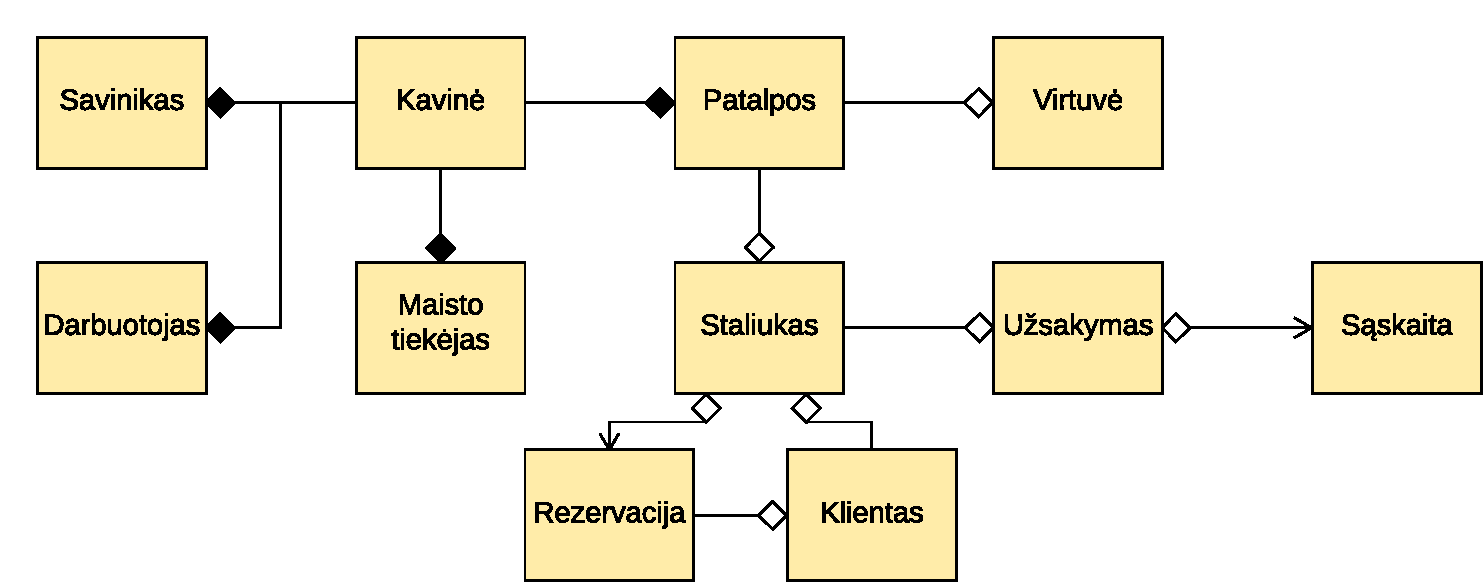
\includegraphics[scale=1]{img/3lab/Diagrama1}
		\caption{Dalykinės srities statinė struktūra}
		\label{fig:diagrama1}
	\end{figure}
\end{landscape}

Pavaizduota diagrama \ref{fig:diagrama1} pav. pavaizduoja kavinės statinę struktūrą. Kavinė negali egzistuoti be maisto tiekėjų (nebus iš ko ruošti maistą),be darbuotojų (nebus galima efektyviai aptarnauti klientų) ir be kavinės savininko, tad šios esybės sudaro kompoziciją, nes viena negali veikti be kitos.\\
Kavinė gali vykti ir be patalpų, kadangi kavinės staliukai gali stovėti ir 
lauke , todėl šie komponentai sudaro agregaciją.\\
Prie  staliuko  neprivalo  sėdėti  klientas,  nes
staliukas  yra  tik  priemonė  aptarnauti ir jam patogiai jaustis restorane,
klientą.Staliukas taip pat gali nebūti rezervuotas, todėl šios esybės sudaro agregaciją.\\
Patalpose gali būti staliukai ir virtuvė, tačiau tai nėra būtina sąlyga, todėl tai sudaro 
agregaciją.\\
Užsakymas konkretizuoja esybę staliukas.\\
Sąskaita seka po to, kai atliekamas užsakymas.\\

\subsection{Užduočių diagrama}
Klientai  yra  agentai,  kurie  naudodamiesi  kavinės  teikiamomis 
paslaugomis  įgyvendina  užduotis - palydėti  atsisėda  prie  staliuko,  atlieka  užsakymus  ir  juos apmoka. \\
Darbuotojas yra agentas, kuris atlieka tokias užduotis kaip palydėti klientą prie staliuko, 
priimti užsakymą, jį paruošti ir priimti apmokėjimą.\\
Maisto tiekėjas yra agentas, kurio užduotis yra pristatyti reikalingas prekes ir produktus kavinei.\\
Kavinės savininkas valdo kavinės išplanavimą ir staliukų išdėstymą kavinėje. Tik kavinės savininkas gali nuspręsti, kur kavinėje bus išdėstomi staliukai.\\
Agentai ir jų užduotys yra pavaizduoti žemiau esančioje dalykinės srities užduočių diagramoje (žr. \ref{fig:diagrama2} pav).\\


	\begin {figure}[H]
	\centering
		
		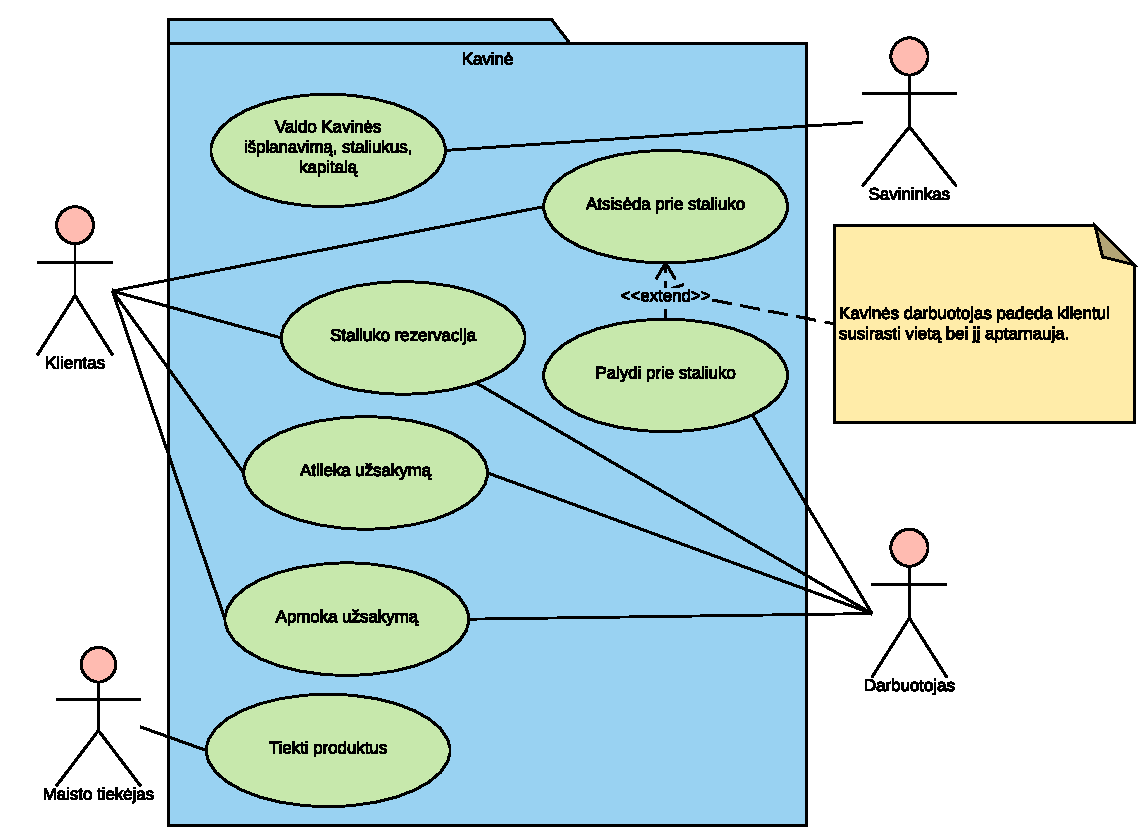
\includegraphics[scale=0.9]{img/3lab/Diagrama2}
		\caption{Dalykinės srities užduočių diagrama}
		\label{fig:diagrama2}
	\end{figure}

\subsection{Užduočių vykdymo scenarijai}
%Insert pauliaus diagram3 here

	\begin {figure}[H]
	\centering
		
		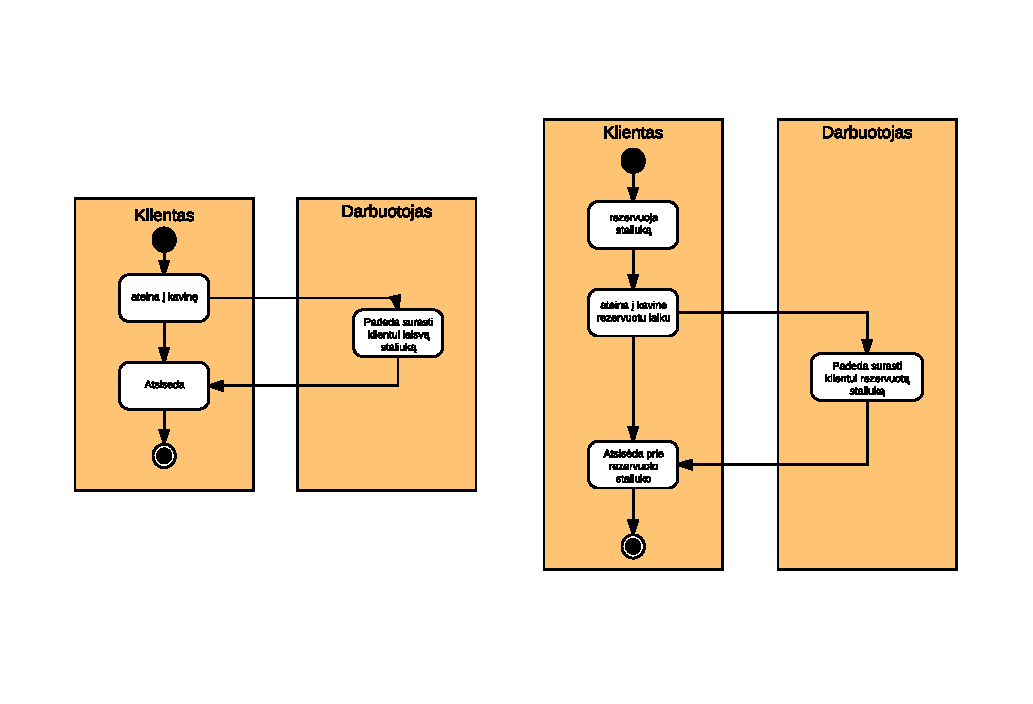
\includegraphics[scale=1]{img/3lab/Diagrama3}
		\caption{Kliento atėjimo į kavinę vykdymo scenarijai}
		\label{fig:diagrama3}
	\end{figure}

Aukščiau pateiktoje užduočių diagramose (žr. \ref{fig:diagrama3} pav.) pavaizduoti kliento be ir su rezervacija užduočių scenarijai.\\ 
Agentas (klientas) ateina į kavinę ir (turėdamas arba neturėdamas rezervacija) gali paprašyti pagalbos darbuotojo,kad padėtų jam rastų staliuką. Klientas gali ir pats susirasti savo staliuką (klientas, neturėdamas rezervacijos, negali atsisėsti į rezervuotą staliuką). \\
Darbuotojas esant poreikiui iš kliento, padeda jam susirasti norimą staliuką: jeigu klientas turi rezervaciją, tai darbuotojas suranda kliento rezervuotą staliuką, jeigu klientas neturi rezervacijos, tai darbuotojas suranda klientui staliuką, kuris nėra rezervuotas tuo metu.\\

%Insert pauliaus diagram4 here

	\begin {figure}[H]
	\centering
		
		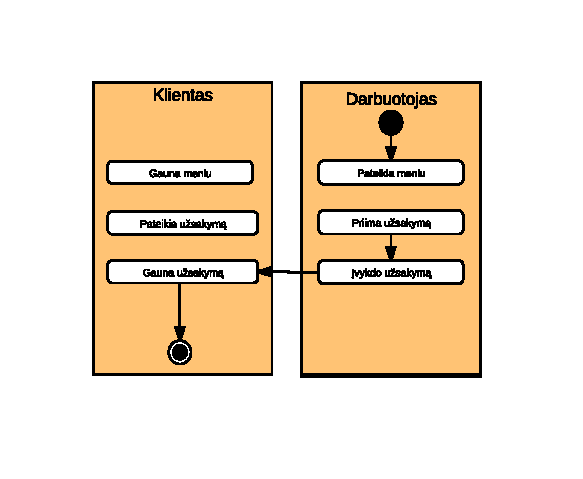
\includegraphics[scale=1]{img/3lab/Diagrama4}
		\caption{kliento aptarnavimo scenarijus}
		\label{fig:diagrama4}
	\end{figure}
Aukšiau pateiktas kliento aptarnavimo vykdymo scenarijus (žr. \ref{fig:diagrama4} pav.). 
Agentas (darbuotojas) pateikia kitam agentui (klientui) meniu. Gavęs meniu, klientas pateikia 
darbuotojui užsakymą ir šis jį priima. Po to, kai priima užsakymą, darbuotojas jį įvykdo ir tuomet klientas gauna įvykdytą užsakymą. \\

%Insert pauliaus diagram5 here
	\begin {figure}[H]
	\centering
		
		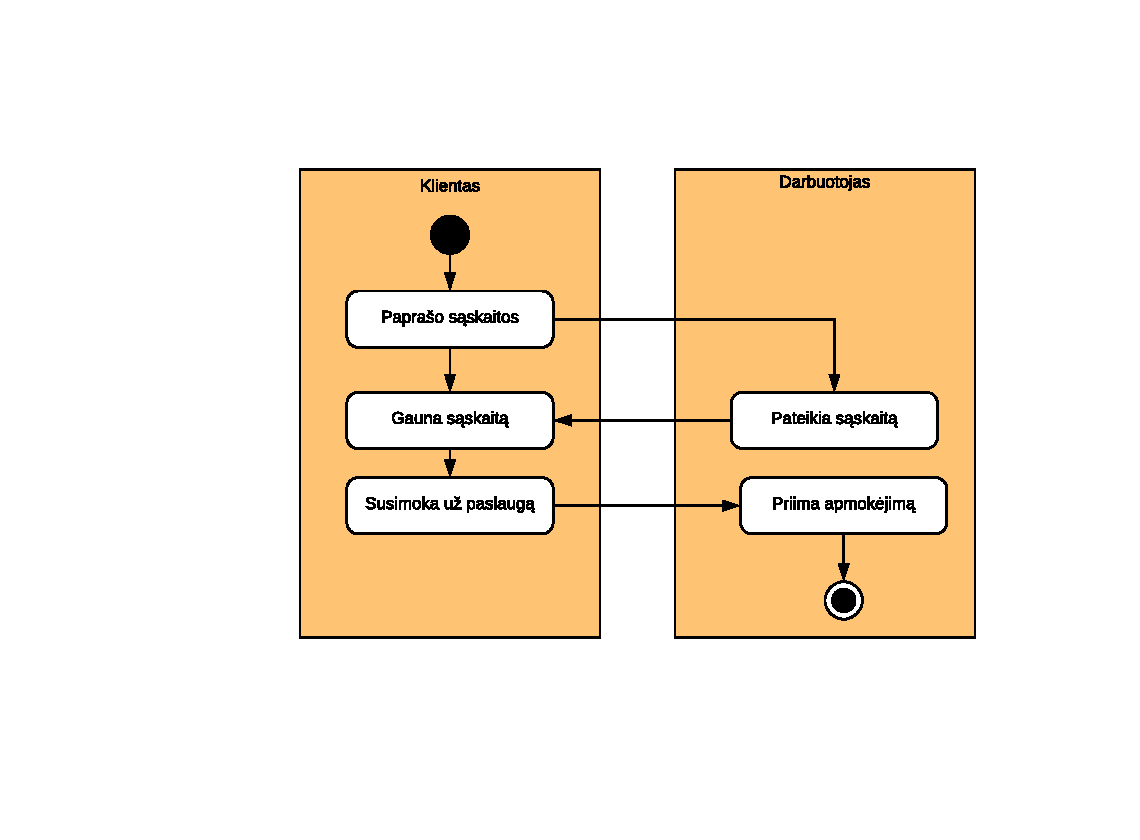
\includegraphics[scale=1]{img/3lab/Diagrama5}
		\caption{kliento atsiskaitymo scenarijus}
		\label{fig:diagrama5}
	\end{figure}
Aukšiau pateiktas kliento atsiskaitymo vykdymo scenarijus (žr. \ref{fig:diagrama5} pav.).
Agentas (klientas) paprašo sąskaitos, tada kitas agentas (darbuotojas) jam ją pateikia. Klientas gauna sąskaitą ir susimoka už jam suteiktas paslaugas. Darbuotojas šį apmokėjimą apdoroja, t.y. jį priima.

%Insert pauliaus diagram 6 here
	\begin {figure}[H]
	\centering
		
		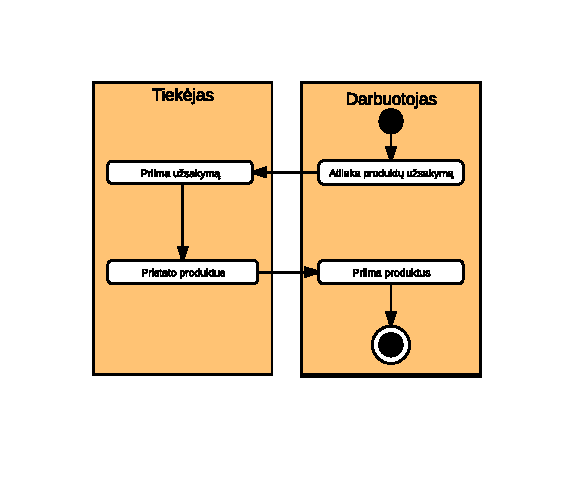
\includegraphics[scale=1]{img/3lab/Diagrama6}
		\caption{Produktų tiekimo į kavinę scenarijus}
		\label{fig:diagrama6}
	\end{figure}
Aukščiau pateiktas reikalingų produktų tiekimo į kavinę scenarijus (žr. \ref{fig:diagrama6} pav.). Agentas (klientas) atlieka kavinei reikiamų produktų užsakymą, tada 
agentas(tiekėjas) jį priima ir pristato produktus. Darbuotojas pristatytus produktus priima. 
\pagebreak
\subsection{Dalykinės srities dinaminė struktūra}

%Insert pauliaus diagram7 here
	\begin {figure}[H]
	\centering
		
		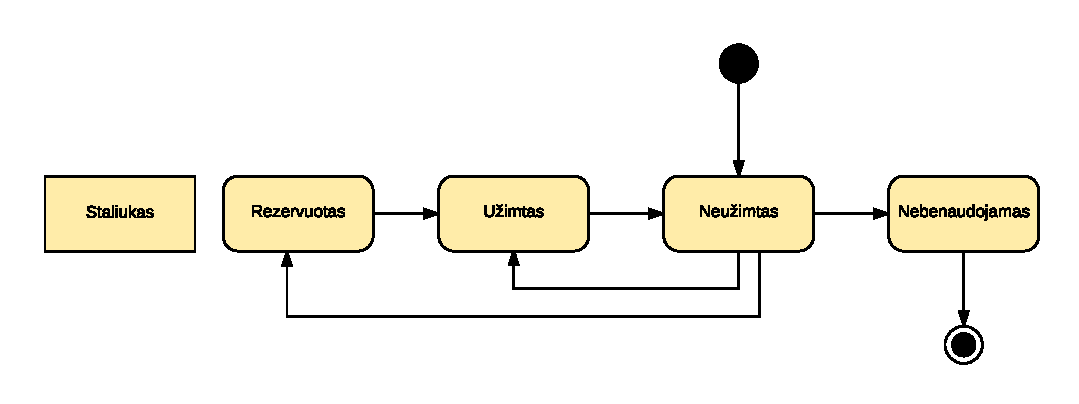
\includegraphics[scale=0.9]{img/3lab/Diagrama7}
		\caption{Staliuko būsenų diagrama}
		\label{fig:diagrama7}
	\end{figure}
		
Pradinė  staliuko  būsena (žr. \ref{fig:diagrama7} pav.)  - neužimtas.  Iš  šios  būsenos  staliukas  gali  tapti  užimtas  arba nebenaudojamas. Iš būsenos užimtas staliukas gali pereiti tik į būseną užimtas. 


%Insert pauliaus diagram8 here

	\begin {figure}[H]
	\centering
		
		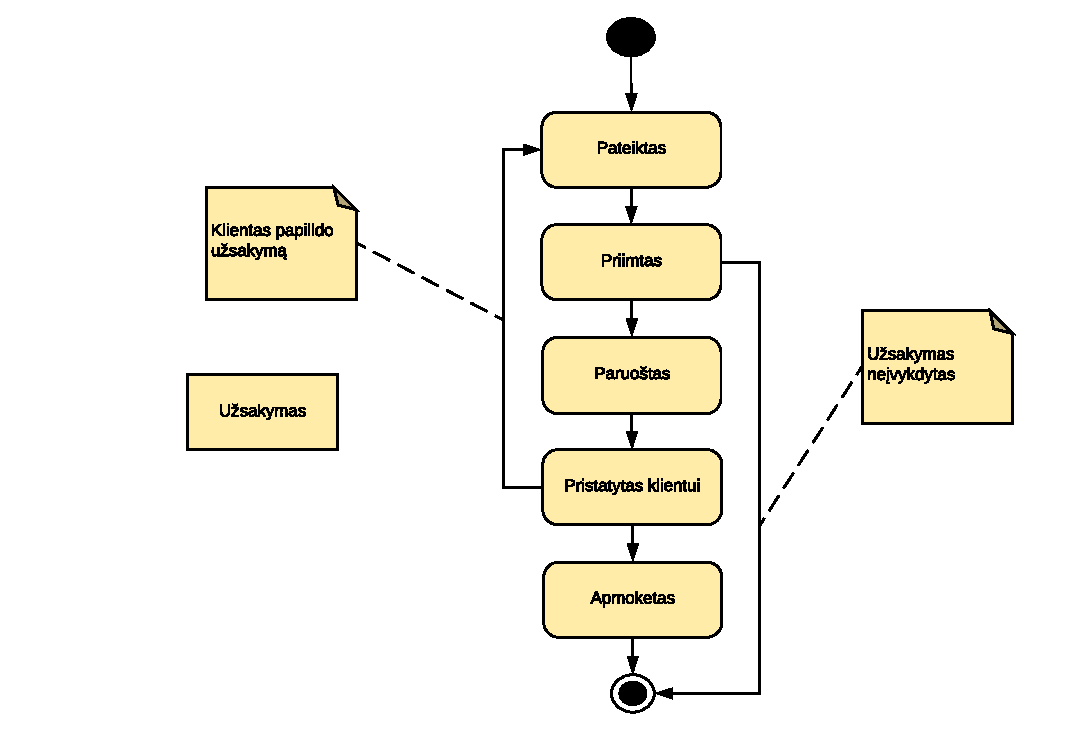
\includegraphics[scale=0.9]{img/3lab/Diagrama8}
		\caption{Užsakymo būsenų diagrama}
		\label{fig:diagrama8}
	\end{figure}

Pradinė užsakymo būsena (žr. \ref{fig:diagrama8} pav.) - “pateiktas”, kadangi užsakymas pradeda egzistuoti, kai klientas jį pateikia darbuotojui. Darbuotojui užsirašius ir perdavus užsakymą virtuvei, jis pereina į būseną “priimtas”. Jei užsakymas neįvykdytas, jis nustoja galioti, kitu atveju užsakymas  tampa “paruoštas”. Paruoštas užsakymas yra pristatomas klientui ir keičia būseną į “pristatytas klientui”. Šis turi galimybę arba užsisakyti ką nors papildomai, arba apmokėti sąskaitą. Kai sąskaita apmokama, būsena pasikeičia į „apmokėtas“.\\
\section{Analizės rezultatai}

Šiame skyriuje vidinė ir išorinė verslo proceso analizė apibendrinama pateikiant esmines įžvalgas SSGG (SWOT) lentelės pavidalu. Lentelėje struktūrizuotai pateikiamos verslo stiprybės, silpnybės, jam kylančios grėsmės ir atsiradusios neišnaudotos galimybės (žr. \ref{fig:diagrama9} pav.).

	\begin {figure}[H]
	\centering
		
		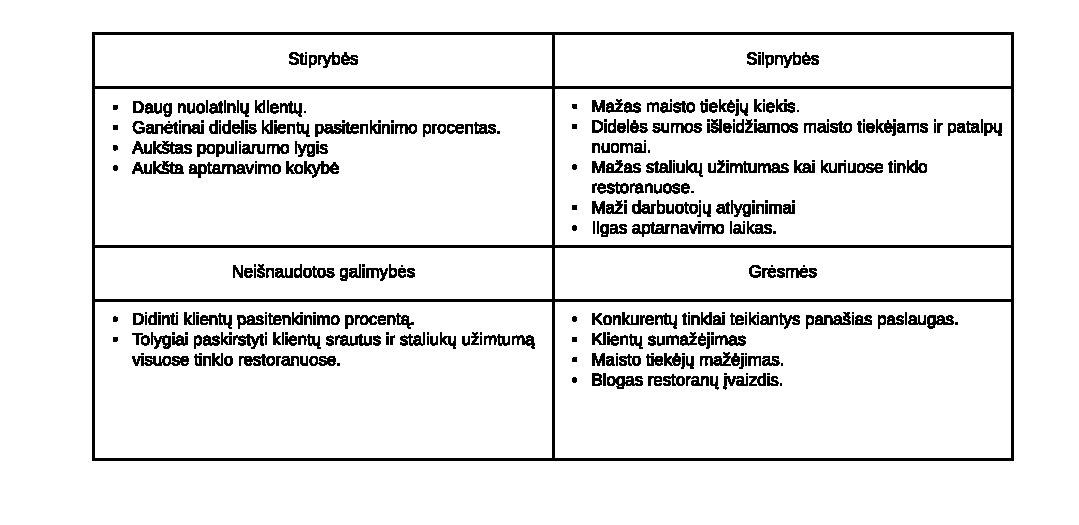
\includegraphics[scale=1]{img/3lab/Diagrama9}
		\caption{SWOT lentelė}
		\label{fig:diagrama9}
	\end{figure}

\section{Verslo proceso tobulinimo strategija}
\noindent \textbf{Vizija}.\\
Visi restorano maisto užsakymo ir tiekimo komponentai(užsakymai vietoje, telefonu, internetu, mobilia programėle, maisto tiekimas vietoje bei į namus) turi atnešti pelno restoranui.\\
\textbf{Misija}.\\
Gerinti maisto tiekimo sąlygas klientams, naudojantis šiuolaikinėmis technologijomis, tobulinti mažiau pelningus komponentus.\\
\textbf{Tikslai/Siekiai}.\\
Didinti restorano staliukų užimtumą, lanksčiai paskirstant klientų srautus:
	\begin{itemize}
	\item Gerinti maisto kokybę ieškaint naujų tiekėjų;
	\item Sumažinti klientų aptarnavimo trukmę;
	\item Pagerinti klientų aptarnavimo kokybę;
	\item Didinti algas restorano darbuotojams;
	\item Didinti klientų užimtumą laukimo metu (plėsti pramogų skaičių, tokių kaip mokami stalo žaidimai ir kt.);
	\end{itemize}
Plėsti užsakymo „iš namų“ sistemą, kuriant internetinę svetainę ar mobilią programėlę, kurios leistų:
	\begin{itemize}
	\item Žemėlapyje parodytų arčiausiai esančius restoranus ir jų laisvų staliukų skaičių;
	\item Matyti restorano staliukų išplanavimą bei kurie staliukai restorane nėra užimti,
	\item Rezervuoti staliuką restorane norimu laiku tam tikroje vietoje;
	\end{itemize}

\section{Sistemos naudojimo scenarijus}

Šiame skyriuje yra aprašyti sistemos teikiama nauda bei žemiau pateiktas sistemos naudojimo scenarijus (žr \ref{fig:maincase} pav.).

% čia reikia imest diagrama MainCase.jpg
\subsection{Naudojimo scenarijus}
	\begin {figure}[H]
	\centering	
		
		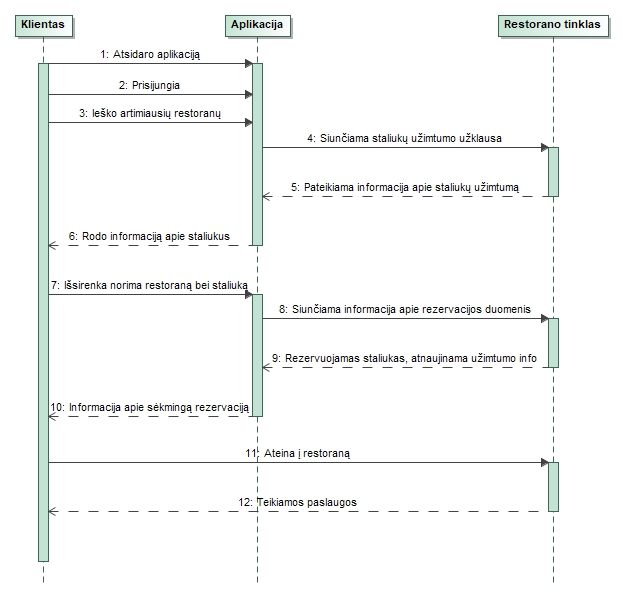
\includegraphics[scale=0.7]{img/3lab/MainCase.jpg}
		\caption{pagrindinis sistemos naudojimo scenarijus}
		\label{fig:maincase}
	\end{figure}
Vartotojas atsidaro mobiliąją aplikaciją, įrašytą išmaniajame telefone arba planšetėje. Ivedęs prisijungimo duomenis jis patenka į pagrindinį langą, kuriame gali ieškoti artimiausiai esančių restoranų pagal vartotojo esamą lokaciją. Aplikacija siunčia užklausą į restoranų tinklą apie restoranų užimtumą. Vartotojui pateikiamas sąrašas restoranų su informacija apie esamus laisvus ir užimtus staliukus. Vartotojas išsirenką jam tinkantį restoraną ir pasirenką staliuką, kurį norėtų rezervuoti. Duomenys apie rezervavimą yra siunčiami restoranų tinklui, kuriame vyksta staliuko rezervavimas ir atnaujinta informacija siunčiama aplikacijai. Vartotojui yra pateikiama informaciją apie sėkmingai rezervuotą staliuką. Jam lieka tik ateiti į restoraną ir jam yra teikiamos paslaugos, kurios buvo numatytos užsakymo informacijoje.

\subsection{Sistemos teikiama nauda}

Žemiau pateiktoje diagramoje yra pavaizduoti sistemos naudojimo privalumai (žr \ref{fig:systemusingbenefits} pav.).
% čia reikia įmest diagramą SystemUsingBenefits.jpg

	\begin {figure}[H]
	\centering	
		
		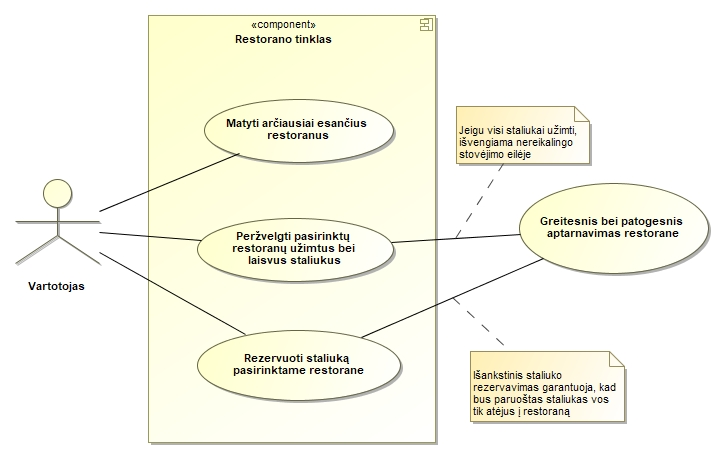
\includegraphics[scale=0.7]{img/3lab/SystemUsingBenefits.jpg}
		\caption{Systemos naudojimo scenarijus}
		\label{fig:systemusingbenefits}
	\end{figure}

Vartotojas gali matyti arčiausiai jo esančius restoranus. Taip pat jis turi galimybę matyti užimtus bei laisvus restoranų staliukus, kas leidžia išvengti bereikalingo stovėjimo eilėje, jeigu visi staliukai užimti. Be šių privalumų, vartotojas gali iš anksto užsirezervuoti staliuką norimame restorane ir užsitikrinti, kad vos tik atvykus į restoraną jam bus paruoštas rezervuotas staliukas bei nereikės laukti.

\subsection{Esama būklė}

Mobiliajai aplikacijai „Covfefe“ realizuoti gali reikėti:
\begin{itemize}
\item Interneto ryšio.
\item Serverio, kuriame būtų saugomi duomenys apie klientus bei staliukų rezervaciją.
\item Restoranų tinkle įdiegtos programinės įrangos, galinčios siųsti duomenis apie restorano staliukų pozicijas bei jų užimtumą.
\item Žmonių, galinčių įdiegti ir tvarkyti sistemą.
\item Mobiliosios aplikacijos.
\end{itemize}


\subsection{Priemonės scenarijui įgyvendinti}

Priemonės, reikalingos sistemos scenarijui įgyvendinti:
\begin{itemize}
\item Interneto priegos.
\item Naujos darbo vietos technikai įtaisyti ir prižiūrėti.
\item Darbuotojų apmokymo.
\item Algoritmo, randančio arčiausiai esančius restoranus su jų laisvų staliukų skaičiais.
\item Duomenų bazės, kurioje būtų saugomos lentelės su klientų informacija bei staliukų rezervacijomis.

\end{itemize}

 \section{Įgyvendinamumo ir naudos analizė}
Šiame skyriuje bus analizuojamas sistemos įgyvendinamumas ir jos nauda.
\subsection{Operacinis įgyvendinamumas}
Inovaciniai slenksčiai:\\
Darbuotojai su žemu kompiuteriniu raštingumu gali nemokėti naudotis nauja programine įranga arba
nenorėti prisitaikyti prie pokyčių.\\
Klientai, nepratę prie naujos aplikacijos, gali nežinoti, kaip ji tiksliai veikia ir ja nesinaudoti.\\
\\
Šių inovacinių slenksčių panaikinimo būdai:\\
Darbuotojams vesti mokymus, paaiškinti apie sistemos teikiama naudą darbuotojams, geriausiai ir
greičiausiai prisitaikiusiems prie naujos aplikacijos mokėti priedus.\\
Naujai aplikacijai sukurti ir taikyti reklamos strategiją\\
Klientams sukūrti demonstracinį video įrašą, kuris supažindins su sistemos pagrindiniais panaudojimo scenarijais.

\subsection{Techninis įgyvendinamumas}
Kompiuteris su Windows OS ir bent:\newline
{\begin{itemize}
\item 2048MB RAM
\item 20GB HDD
\item 1700MHz procesoriumi
\end{itemize}

\subsection{Ekonominis įgyvendinamumas}
Reikalinga techninė įranga (serveriui):
{\begin{itemize}
\item Kompiuteris - 1000 eur
\item Nepertraukiamo maitinimo šaltinis - 180 eur
\item Tinklo įranga - 30 eur
\item Iš viso: 1210 eur
\end{itemize}
\hfill\break


Reikalinga techninė įranga (vienam restoranui):

{\begin{itemize}
\item Kompiuteris - 500 eur 
\item Nepertraukiamo maitinimo šaltinis - 180 eur
\item Iš viso: 680 eur
\end{itemize}
\break

Programinė įranga:
{\begin{itemize}
\item Operacinė sistema Windows 10 Pro - 200 eur 
\item Sistema „Covfefe“ - 10 000 eur
\item Iš viso: 10 200 eur
\end{itemize}
\hfill\break

Bendra įrangos kaina - 12 090 eur

Metinės eksplotavimo išlaidos:
{\begin{itemize}
\item Atlyginimas sistemos administratoriui - 7 200 eur
\item Interneto paslaugos - 1000 eur
\item Programinės ir techninės įrangos aptarnavimas ir atnaujinimas - 5000 eur
\item Iš viso: 13200 eur per metus
\end{itemize}
\hfill\break

Numanoma verslui atnešama nauda:\\
Registruotose restoranuose (orientuojamasi į 60 registruotų restoranų tinklą) apsilanko 250000 žmonių per mėnesį. Per metus registruotu restoranų tinklas gauna 600000
eur pelno.\\
Įdiegus sistemą “Covfefe” tikimasi padidinti staliukų užimtumą 15\% ir taip padidinti
pelną 90000 eur per metus.
\hfill\break

Sistema atsipirktų po 8 menėsių. 

\subsection{Juridinis įgyvendinamumas}
Sukuriant sistemą nebus pažeista Lietuvos respublikos konstitucija, Asmens duomenų
apsaugos įstatymas, Statistikos įstatymas ar kitų Lietuvos Respublikos teisės aktų numatyti
draudimai.\\
 Darbuotojai turi teisę į tinkamas, saugias ir sveikas darbo sąlygas. Darbuotojams
mokamas menėsinis atlyginimas, darbo valandos neviršija 8 valandų per parą. Kiekvienas
darbuotojas turi teisę į poilsį ir laisvalaikį, taip pat kasmetines mokamas atostogas.\\ 
Duomenys tvarkomi tiksliai, sąžiningai ir konfidencialiai.
\break

%FUNKCINIAI REIKALAVIMAI

\section{Vartotojo sąsaja}
Šiame skyriuje pateikiamos formuluojamos užduotys, jų formulavimo kalbos ir protokolo reikalavimai, taip pat interfeiso darnos ir standartizavimo, pranešimų formulavimo bei interfeiso individualizavimo reikalavimai.
 
\subsection{Formuluojamos užduotys}
Šiame poskyryje pateikiamos kliento ir kavinės savininko užduotys. užduotis atitinkantys pavyzdžiai: žr. ~\ref{fig:b} pav. ir ~\ref{fig:c} pav.
\subsubsection{Kliento užduotys}
\begin{center}
	\begin{table}[H]
	\caption{Kliento užduotys}
	\begin{tabular}{|p{2cm}|p{2,5cm}|p{9,6cm}|}
	\hline
	    \rowcolor{lightgray}
		\multicolumn{3}{|c|}{Kliento užduotys}\\
		
	\hline
		\multicolumn{1}{|c|}{{\bfseries Kodas}}&
		\multicolumn{1}{|c|}{{\bfseries Užduotis}}&
		\multicolumn{1}{|c|}{{\bfseries Formulavimo būdas}}\\		
	\hline
		\multicolumn{1}{|c|}{VS 1}& 	
		\multicolumn{1}{|c|}{Autentifikavimo užduotys}&
		{
			\begin{enumerate}
				\item Registruotis sistemoje
				(privalomi duomenys:vardas, pavardė, el. paštas, telefono numeris, slaptažodis).
				\item Prisijungti prie sistemos (privalomi duomenys: el. paštas, slaptažodis).
				\item “Premium” prisijungimas (aktyvuojamas klientui, kuris nupirko tam tikrą paslaugą), leidžiantis prisijungti prie sistemos vienu mygtuko paspaudimu.
			\end{enumerate}}\\
	
	\hline
		\multicolumn{1}{|c|}{VS 2}&  	
		\multicolumn{1}{|c|}{Pagalbinės užduotys}&
		{
			\begin{enumerate}
				\item Peržiūrėti visas sistemoje registruotas kavinės, informaciją apie jas.
				\item Ieškoti kavinės pagal vardą.
				\item Ieškoti kavinės pagal vietą.
				\item Peržiūrėti pasirinktos kavinės detalią informaciją (Vardas, adresas, staliukų skaičius, darbo grafikas).
				\item Rezervuoti staliuką pasirinktoje kavinėje.
			\end{enumerate}}\\
	
	\hline 	 	
	\end{tabular}

	\label{table:1}
	\end{table}

\end{center}

\subsubsection{Kavinės savininko užduotys}
\begin{center}
	\begin{table}[H]
	\caption{Kavinės savininko užduotys}
	\begin{tabular}{|p{2cm}|p{2,5cm}|p{9,6cm}|}
	\hline
	    \rowcolor{lightgray}
		\multicolumn{3}{|c|}{Kavinės savininko užduotys}\\
		
	\hline
		\multicolumn{1}{|c|}{{\bfseries Kodas}}&
		\multicolumn{1}{|c|}{{\bfseries Užduotis}}&
		\multicolumn{1}{|c|}{{\bfseries Formulavimo būdas}}\\		
	\hline
		\multicolumn{1}{|c|}{VS 3}&  	
		\multicolumn{1}{|c|}{Autentifikavimo užduotys}&
		{
			\begin{enumerate}
				\item Registruotis sistemoje (privalomi duomenys: vardas, pavardė, el. paštas, telefono numeris, slaptažodis).
				\item Prisijungti prie sistemos (privalomi duomenys: el. paštas, slaptažodis).
			\end{enumerate}}\\
	\hline
		\multicolumn{1}{|c|}{VS 4}&
		\multicolumn{1}{|c|}{Pagalbinės užduotys}&
		{
			\begin{enumerate}
				\item Pridėti kavinę (privalomi duomenys: kavinės vardas, adresas, staliukų skaičius, darbo grafikas. Papildomi: kavinės telefono numeris).
				\item Peržiūrėti sistemoje registruotų kavinių sąrašą.
				\item Atnaujinti informaciją apie savo registruotą kavinę.
			\end{enumerate}}\\
	
	\hline 	 	
	\end{tabular}
	
	\label{table:2}
	\end{table}

\end{center}

\subsection{Užduočių formulavimo kalbos reikalavimai}
\begin{center}

	\begin{longtable}{|p{2cm}|p{4,1cm}|p{9,6cm}|}
	\caption{Užduočių formulavimo kalbos reikalavimai}
	\label{table:3}	
	\endfirsthead
	\endhead
	\hline
	    \rowcolor{lightgray}
		\multicolumn{3}{|c|}{Užduočių formulavimo kalbos reikalavimai}\\
		
	\hline
		\multicolumn{1}{|c|}{{\bfseries Kodas}}&
		\multicolumn{1}{|c|}{{\bfseries Užduotis}}&
		\multicolumn{1}{|c|}{{\bfseries Formulavimo būdas}}\\		
	\hline
		\multicolumn{1}{|c|}{VS 5}& 	
		{Registruotis}&
		\multicolumn{1}{|p{8,6cm}|}{
			\begin{enumerate}
				\item Duomenų įvedimo laukeliai.
				\item Registracijos mygtukas.
			\end{enumerate}}\\
	
	\hline
		\multicolumn{1}{|c|}{VS 6}& 	
		{Prisijungti}&
		\multicolumn{1}{|p{8,6cm}|}{
			\begin{enumerate}
				\item Piktrograma. 
				\item Duomenų įvedimo laukeliai.
				\item Prisijungimo  mygtukas.
			\end{enumerate}}\\
	
	\hline
		\multicolumn{1}{|c|}{VS 7}& 	
		{Premium prisijungimas}&
		\multicolumn{1}{|p{8,6cm}|}{
			\begin{enumerate}
				\item Premium prisijungimo mygtukas.
			\end{enumerate}}\\
	
	\hline
		\multicolumn{1}{|c|}{VS 8}& 	
		{Kavinės pridėjimas}&
		\multicolumn{1}{|p{8,6cm}|}{
			\begin{enumerate}
				\item Duomenų įvedimo laukeliai.
				\item Pridėjimo mygtukas.
			\end{enumerate}}\\
	
	\hline 	
		\multicolumn{1}{|c|}{VS 9}&
		\multicolumn{1}{|c|}{Išeiti}&
		\multicolumn{1}{|p{8,6cm}|}{
			\begin{enumerate}
				\item Išėjimo mygtukas.
			\end{enumerate}}\\
	
	\hline	
		\multicolumn{1}{|c|}{VS 10}&
		{Kavinės paieška}&
		\multicolumn{1}{|p{9,2cm}|}{
			\begin{enumerate}
				\item Lentelė su sistemoje registruotomis kavinėmis.
				\item Kavinės rezervacijos mygtukas.
				\item Paieškos duomenų įvedimo laukelis.
				\item Paieškos pagal vardą mygtukas.
				\item Paieškos pagal vietą mygtukas.
				\item Parodyti daugiau informacijos mygtukas.
			\end{enumerate}}\\
	
	\hline 	
		\multicolumn{1}{|c|}{VS 11}&
		{Kavinės rezervacija}&
		\multicolumn{1}{|p{9,2cm}|}{
			\begin{enumerate}
				\item Datos (metai, mėnuo, diena) nustatymo laukelis.
				\item Laiko (valandos, minutės) nustatymo laukelis.
				\item Lango uždarymo mygtukas.
				\item Rezervacijos mygtukas.
			\end{enumerate}}\\
	
	\hline
		\multicolumn{1}{|c|}{VS 12}& 	
		{Kavinės informacijos atnaujinimas}&
		\multicolumn{1}{|p{8,6cm}|}{
			\begin{enumerate}
				\item Duomenų įvedimo laukeliai.
				\item Patvirtinimo mygtukas.
			\end{enumerate}}\\
	
	\hline
	
	
	\end{longtable}

\end{center}

\pagebreak

\begin{landscape}
\subsection{Užduočių formulavimo būdo(protokolo) reikalavimai}
	\begin {figure}[H]
		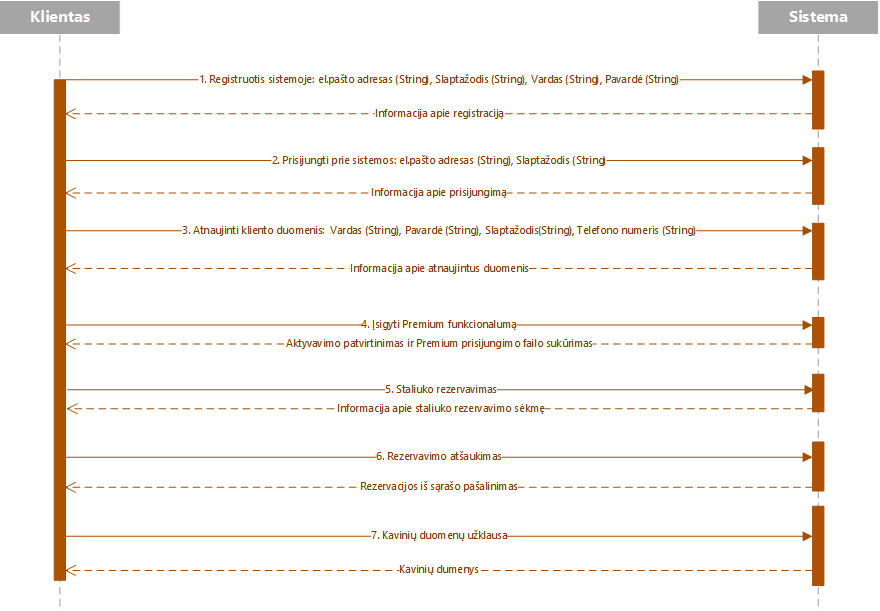
\includegraphics[width=1.2\textwidth,height=1.3\textheight,keepaspectratio]{img/b}
		\caption{Kliento ir sistemos užduotys}
		\label{fig:b}
	\end{figure}
\end{landscape}

\begin{landscape}
	\begin {figure}[H]
		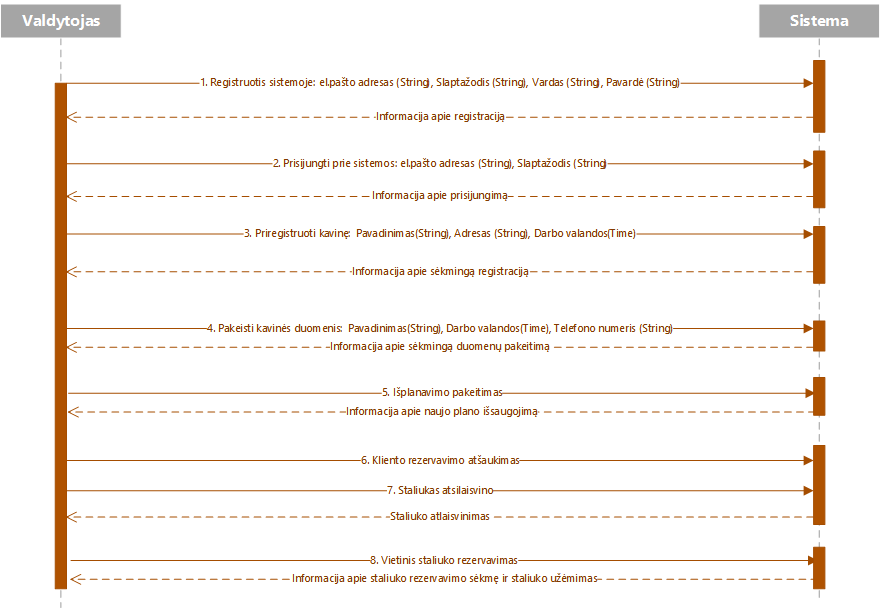
\includegraphics[width=1.3\textwidth,height=1.4\textheight,keepaspectratio]{img/c}
		\caption{Kavinės savininko ir sistemos užduotys}
		\label{fig:c}
	\end{figure}
\end{landscape}


\subsection{Interfeiso darnos ir standartizavimo reikalavimai}
\begin{center}
	\begin{table}[H]
	\caption{Interfeiso darnos ir standartizavimo reikalavimai}
	\begin{tabular}{|p{2cm}|p{14cm}|p{2cm}|}
	\hline
	    \rowcolor{lightgray}
	    \multicolumn{3}{|c|}{Interfeiso darnos ir standartizavimo reikalavimai}\\
	\hline
		\multicolumn{1}{|c|}{{\bfseries Kodas}}&
		\multicolumn{1}{|c|}{ {\bfseries Užduotis}}&
		\multicolumn{1}{|c|}{{\bfseries Svarba}}\\		
	\hline
		\multicolumn{1}{|c|}{VS 13}&
		\multicolumn{1}{|p{12,9cm}|}{Pagrindinis meniu visuomet pasiekiamas paspaudus ant programėlės logotipo, esančio kairiajame viršutiniame kampe.}& 
		\multicolumn{1}{|p{1.5cm}|}{PAGEIDAUTINA}\\
	\hline
		\multicolumn{1}{|c|}{VS 14}&
		\multicolumn{1}{|p{12cm}|}{Languose dominuoja „Royal Jewels“ spalvų paletė.}& 
		\multicolumn{1}{|p{1.5cm}|}{PAGEIDAUTINA}\\
	\hline
		\multicolumn{1}{|c|}{VS 15}&
		\multicolumn{1}{|p{12cm}|}{Tekstui naudojami ‚Times New Roman“ šriftas}& 
		\multicolumn{1}{|p{1.5cm}|}{PAGEIDAUTINA}\\
	\hline  	 	
	
	\end{tabular}
	
	\label{table:4}
	\end{table}

\end{center}

\subsection{Pranešimų formulavimo reikalavimai}
\begin{center}
	\begin{table}[H]
	\caption{Pranešimų formulavimo reikalavimai}
	\begin{tabular}{|p{2cm}|p{11cm}|p{2cm}|}
	\hline
	    \rowcolor{lightgray}
	    \multicolumn{3}{|c|}{Pranešimų formulavimo reikalavimai}\\
	\hline
		\multicolumn{1}{|c|}{{\bfseries Kodas}}&
		\multicolumn{1}{|c|}{ {\bfseries Užduotis}}&
		\multicolumn{1}{|c|}{{\bfseries Svarba}}\\		
	\hline
		\multicolumn{1}{|c|}{VS 16}&
		\multicolumn{1}{|p{12,6cm}|}{Pranešimų tekstas turi būti parašytas laikantis gramatikos ir skyrybos taisyklių.}& 
		\multicolumn{1}{|c|}{BŪTINA}\\
	\hline
		\multicolumn{1}{|c|}{VS 17}&
		\multicolumn{1}{|p{12,5cm}|}{Pranešime vartojami tik interfeiso naudotojams žinomi terminai, vengiama žargonų ir svetimybių, tačiau leistina vartoti dalykinės srities metaforas.}& 
		\multicolumn{1}{|c|}{BŪTINA}\\
	\hline
		\multicolumn{1}{|c|}{VS 18}&
		\multicolumn{1}{|p{12,5cm}|}{Informacinio tipo pranešimai aprašys domenų įvedimo kriterijus.}& 
		\multicolumn{1}{|c|}{BŪTINA}\\
	\hline
		\multicolumn{1}{|c|}{VS 19}&
		\multicolumn{1}{|p{12,5cm}|}{Pranešimų langai įspės apie blogai įvestus duomenis, pavyzdžiui, per trumpą įvestą slaptažodį arba jau užregistruotą el. paštą.}& 
		\multicolumn{1}{|c|}{BŪTINA}\\
	\hline
		\multicolumn{1}{|c|}{VS 20}&
		\multicolumn{1}{|p{12,5cm}|}{Pranešimas turi informuoti apie sėkmingai arba nesėkmingai atliktą veiksmą.}& 
		\multicolumn{1}{|c|}{BŪTINA}\\
	\hline
		\multicolumn{1}{|c|}{VS 21}&
		\multicolumn{1}{|p{12,5cm}|}{Pranešimo tekstas turi būti suprantamas vienareikšmiškai.}& 
		\multicolumn{1}{|c|}{BŪTINA}\\
	\hline
		\multicolumn{1}{|c|}{VS 22}&
		\multicolumn{1}{|p{12,5cm}|}{Pranešimas apie klaidą turi būti detalus.}& 
		\multicolumn{1}{|p{1.5cm}|}{PAGEIDAUTINA}\\
	\hline
		\multicolumn{1}{|c|}{VS 23}&
		\multicolumn{1}{|p{12,5cm}|}{Informacinis pranešimas turi būti žalios arba mėlynos spalvos, o klaidos pranešimas - raudonos.}& 
		\multicolumn{1}{|p{1.5cm}|}{PAGEIDAUTINA}\\
	\hline
		\multicolumn{1}{|c|}{VS 24}&
		\multicolumn{1}{|p{12,5cm}|}{Pradinis pranešimo langas negali užimti daugiau nei 50\% ekrano pločio ir aukščio.}& 
		\multicolumn{1}{|p{1.5cm}|}{PAGEIDAUTINA}\\
	\hline
		\multicolumn{1}{|c|}{VS 25}&
		\multicolumn{1}{|p{12,5cm}|}{Pranešimo teksto ilgis negali viršyti 100 simbolių limito.}& 
		\multicolumn{1}{|p{1.5cm}|}{PAGEIDAUTINA}\\
	\hline
		\multicolumn{1}{|c|}{VS 26}&
		\multicolumn{1}{|p{12,5cm}|}{Pranešimas turi turėti antraštę.}& 
		\multicolumn{1}{|p{1.5cm}|}{PAGEIDAUTINA}\\
	\hline
		\multicolumn{1}{|c|}{VS 27}&
		\multicolumn{1}{|p{12,5cm}|}{Turi būti galimybė išjungti pranešimo langą.}& 
		\multicolumn{1}{|c|}{BŪTINA}\\
	\hline	 	
	
	\end{tabular}
	
	\label{table:5}
	\end{table}

\end{center}

\pagebreak

\subsection{Interfeiso individualizavimo reikalavimai}

\begin{center}
	\begin{table}[H]
	\caption{Interfeiso individualizavimo reikalavimai}
	\begin{tabular}{|p{2cm}|p{13cm}|p{2cm}|}
	\hline
	    \rowcolor{lightgray}
	    \multicolumn{3}{|c|}{Interfeiso individualizavimo reikalavimai}\\
	\hline
		\multicolumn{1}{|c|}{ {\bfseries Kodas}}&
		\multicolumn{1}{|c|}{ {\bfseries Užduotis}}&
		\multicolumn{1}{|c|}{{\bfseries Svarba}}\\		
	\hline
		\multicolumn{1}{|c|}{VS 28}&
		\multicolumn{1}{|p{12,9cm}|}{Ekrano temos pasirinkimas (minimalūs dizaino pakeitimai: spalva, šriftas)}& 
		\multicolumn{1}{|p{1.5cm}|}{PAGEIDAUTINA}\\
	\hline
		\multicolumn{1}{|c|}{VS 29}&
		\multicolumn{1}{|p{12,9cm}|}{Kalbos pasirinkimas.}& 
		\multicolumn{1}{|p{1.5cm}|}{PAGEIDAUTINA}\\
	\hline
	
	\end{tabular}
	
	\label{table:6}	
	\end{table}
\end{center}

\section{Funkciniai reikalavimai}
%PRADEDAME RASYTI LENTELES WOHOO

Šiame skyriuje pateikiami aplikacijos funkciniai reikalavimai ir jų įgyvendinimo svarba.

\subsection{Aplikacijos langai}

 %APLIKACIJOS LANGAI
\begin{center}
	\begin{table}[H]
	\caption{Aplikacijos langų funkciniai reikalavimai.}
	\begin{tabular}{|p{2cm}|p{12,5cm}|p{3,5cm}|}
	\hline
	    \rowcolor{lightgray}
		\multicolumn{3}{|c|}{Aplikacijos langai}\\
		
	\hline
		\multicolumn{1}{|c|}{{\bfseries Kodas}}&
		\multicolumn{1}{|c|}{{\bfseries Reikalavimas}}&
		\multicolumn{1}{|c|}{{\bfseries Svarba}}\\

	\hline
		\multicolumn{1}{|c|}{FR 1} &
		Iš visų aplikacijos langų galima grįžti į prisijungimo langą &
		\multicolumn{1}{|c|}{BŪTINA}\\
	\hline
		\multicolumn{1}{|c|}{FR 2} &
		{Visi langai po prisijungimo turi turėti galimybę parodyti kliento \newline prisijungimo vardą/paštą.}&
		\multicolumn{1}{|c|}{BŪTINA}\\
	\hline
	
		\multicolumn{1}{|c|}{FR 3}&
		{Jeigu klientas turi rezervavęs staliuką - iš visų langų, išskyrus \newline prisijungimo, galima patekti į langą, rodantį rezervacijos informaciją.}&
		\multicolumn{1}{|c|}{BŪTINA}\\
	\hline
		\multicolumn{1}{|c|}{FR 4}&
		{Iš prisijungimo lango galima patekti į registracijos ir meniu langą.}&
		\multicolumn{1}{|c|}{BŪTINA}\\
	\hline
		\multicolumn{1}{|c|}{FR 5}&
		{Iš meniu lango galima patekti į:\newline
		\begin{enumerate}
			\item Jei prisijungia kavinės administratorius:
				\begin{enumerate}
					\item “Keisti kavinės informaciją” langą.
					\item “Keisti kavinės išplanavimą” langą.
				\end{enumerate}
			\item Jei prisijungia kavinės darbuotojas:
				\begin{enumerate}
					\item “Lokali rezervacija” langą.
				\end{enumerate}
			\item Jei prisijungia klientas:
				\begin{enumerate}
					\item “Kavinės paieška” langas.
				\end{enumerate}
			\item Visi prisijungę klientai turi galimybę patekti į “Keisti kliento duomenis” langą.
			\item Visi langai turi turėti galimybę grįžti į ankstesnį langą.
		\end{enumerate}
		}&
		\multicolumn{1}{|c|}{BŪTINA}\\		
	\hline
	
	\end{tabular}
	
	\label{table:AplikacijosLangai}
	\end{table}
	
\end{center}

\pagebreak

\subsection{Kliento registracija}
%Vartotojo prisijungimas
\begin{center}

	\begin{table}[H]
	\caption{Kliento registracijos funkciniai reikalavimai}
	\begin{tabular}{|p{2cm}|p{12,5cm}|p{3,5cm}|}
	\hline
	    \rowcolor{lightgray}
		\multicolumn{3}{|c|}{Kliento registracija}\\
		
	\hline
		\multicolumn{1}{|c|}{{\bfseries Kodas}}&
		\multicolumn{1}{|c|}{{\bfseries Reikalavimas}}&
		\multicolumn{1}{|c|}{{\bfseries Svarba}}\\

	\hline
	\multicolumn{1}{|c|}{FR 6}&
	{Klientas, norintis registruotis prie aplikacijos, turi nurodyti:
		\begin{itemize}
			\item Vardą.
			\item Pavardę.
			\item Slaptažodį.
			\item Telefono numerį (neprivaloma).
			\item Elektroninį paštą.
		\end{itemize}}&		
	\multicolumn{1}{|c|}{BŪTINA}\\
	\hline
	
		\multicolumn{1}{|c|}{FR 7}&
		{Informuoti klientą apie sėkmingą registraciją}&
		\multicolumn{1}{|c|}{BŪTINA}\\	
	\hline
		\multicolumn{1}{|c|}{FR 8}&
		{Kliento duomenys išsaugomi duomenų bazėje}&
		\multicolumn{1}{|c|}{BŪTINA}\\	
	\hline	
		\multicolumn{1}{|c|}{FR 9}&
		{Tam, kad įvestas kliento el. pašto adresas būtų tinkamos formos, jis turi būti sudarytas iš abonento vardo, „@“ simbolio bei domeno adreso.}&
		\multicolumn{1}{|c|}{BŪTINA}\\	
	\hline
		\multicolumn{1}{|c|}{FR 10}&
		{Slaptažodis privalo būti sudarytas bent iš 8 simbolių, turėti bent vieną skaitmenį.
}&
		\multicolumn{1}{|c|}{BŪTINA}\\		
	\hline
		\multicolumn{1}{|c|}{FR 11}&
		{Duomenų bazėje išsaugomi kliento duomenys turi būti string tipo }&
		\multicolumn{1}{|p{1.5cm}|}{PAGEIDAUTINA}\\		
	\hline
	
	\end{tabular}
	
	\label{table:VartotojoRegistracija}
	\end{table}

\end{center}

\subsection{Kliento prisijungimas}

\begin{center}
	\begin{table}[H]
	\caption{Kliento prisijungimo funkciniai reikalavimai}
	\begin{tabular}{|p{2cm}|p{12,5cm}|p{3,5cm}|}
	\hline
	    \rowcolor{lightgray}
		\multicolumn{3}{|c|}{Kliento prisijungimas}\\
		
	\hline
		\multicolumn{1}{|c|}{{\bfseries Kodas}}&
		\multicolumn{1}{|c|}{{\bfseries Reikalavimas}}&
		\multicolumn{1}{|c|}{{\bfseries Svarba}}\\

	\hline
	
		\multicolumn{1}{|c|}{FR 12}&
		{Klientas, norintis prisijungti prie aplikacijos turi nurodyti:
			\begin{itemize}
				\item Elektroninio pašto adresas.
				\item Slaptažodis.
			\end{itemize}
		}&
		\multicolumn{1}{|c|}{BŪTINA}\\	
		
	\hline	
		\multicolumn{1}{|c|}{FR 13}&
		{Klientas prijungiamas prie sistemos ir nukreipiamas į meniu langą kartu su papildomais kliento duomenimis.}&
		\multicolumn{1}{|c|}{BŪTINA}\\
		
	\hline	
		\multicolumn{1}{|c|}{FR 14}&
		{Jei prisijungimo duomenys neteisingi, klientas informuojamas pranešimu.}&
		\multicolumn{1}{|c|}{BŪTINA}\\		
		
	\hline
		\multicolumn{1}{|c|}{FR 15}&
		{Kliento įvesti duomenys (slaptažodis bei el. pašto adresas) turi būti sutikrinti su duomenimis, esančiais duomenų bazėje.}&
		\multicolumn{1}{|c|}{BŪTINA}\\
		
	\hline	
		\multicolumn{1}{|c|}{FR 16}&
		{Jei prisijungimo duomenys neteisingi, klientas informuojamas pranešimu.}&
		\multicolumn{1}{|c|}{BŪTINA}\\
	\hline
	
	
	
	\end{tabular}	
	
	\label{table:VartotojoPrisijungimas}		
	\end{table}

\end{center}
\pagebreak

\subsection{Kavinės pasirinkimas}

\begin{center}
	\begin{table}[H]
	\caption{Kavinės pasirinkimo funkciniai reikalavimai}
	\begin{tabular}{|p{2cm}|p{12,5cm}|p{3,5cm}|}
	
	\hline
	    \rowcolor{lightgray}
		\multicolumn{3}{|c|}{Kavinės pasirinkimas}\\
		
	\hline
		\multicolumn{1}{|c|}{{\bfseries Kodas}}&
		\multicolumn{1}{|c|}{{\bfseries Reikalavimas}}&
		\multicolumn{1}{|c|}{{\bfseries Svarba}}\\

	\hline
	
		\multicolumn{1}{|c|}{FR 17}&
		{Klientui pateikiamas arčiausiai jo esančių kavinių sąrašas kartu su jų duomenimis (ne visais):
		\begin{itemize}
			\item Pavadinimas.
			\item Adresas.
			\item Reitingas.
		\end{itemize}}&
		\multicolumn{1}{|c|}{BŪTINA}\\	
		
	\hline
	
		\multicolumn{1}{|c|}{FR 18}&
		{Klientas gali paspausti ir pasirinkti vieną iš kavinių.}&
		\multicolumn{1}{|c|}{BŪTINA}\\
		
	\hline
	
		\multicolumn{1}{|c|}{FR 19}&
		{Klientui pasirinkus kavinę, parodoma visa jos informacija:
		\begin{itemize}
			\item Pavadinimas.
			\item Adresas.
			\item Vietų skaičius.
			\item Laivų vietų skaičius.
			\item Reitingas.
			\item Darbo valandos.
		\end{itemize}}&
		\multicolumn{1}{|c|}{BŪTINA}\\
		
	\hline
	
		\multicolumn{1}{|c|}{FR 20}&
		{Klientas pasirinkęs kavinę (turinčią laisvų vietų) gali užsisakyti staliuką.}&
		\multicolumn{1}{|c|}{BŪTINA}\\
	\hline
	
		\multicolumn{1}{|c|}{FR 21}&
		{Jeigu klientas nori užsisakyti staliuką, jis yra nukreipiamas į staliuko užsakymo langą}&
		\multicolumn{1}{|c|}{BŪTINA}\\				
	\hline
	
	\end{tabular}		
	
	\label{table:KavinėsPasirinkimas}
	\end{table}


\end{center}

\pagebreak


\subsection{Staliuko užsakymas}
\begin{center}
	\begin{table}[H]
	\caption{Staliuko užsakymo funkciniai reikalavimai.}
	\begin{tabular}{|p{2cm}|p{12,5cm}|p{3,5cm}|}
	
	\hline
	    \rowcolor{lightgray}
		\multicolumn{3}{|c|}{Staliuko užsakymas}\\
		
	\hline
		\multicolumn{1}{|c|}{{\bfseries Kodas}}&
		\multicolumn{1}{|c|}{{\bfseries Reikalavimas}}&
		\multicolumn{1}{|c|}{{\bfseries Svarba}}\\

	\hline
	
		\multicolumn{1}{|c|}{FR 22}&
		{Klientui pateikiamas kavinės išplanavimas su staliukais.}&
		\multicolumn{1}{|c|}{BŪTINA}\\				
	\hline
	
		\multicolumn{1}{|c|}{FR 23}&
		{Klientas pasirinkęs vieną iš laisvų staliukų nukreipiamas į langą, kuriame prašo įvesti rezervacijos datą ir laiką.}&
		\multicolumn{1}{|c|}{BŪTINA}\\				
	\hline
	
		\multicolumn{1}{|c|}{FR 24}&
		{Jei klientas nėra Premium ir kavinėje likęs tik vienas laisvas staliukas, tai jis negali to staliuko rezervuoti ir gauna pranešimą, kad neturi Premium privilegijų.}&
		\multicolumn{1}{|c|}{BŪTINA}\\				
	\hline
	
		\multicolumn{1}{|c|}{FR 25}&
		{Klientas norėdamas rezervuoti vietą restorane privalo nurodyti:
			\begin{itemize}
				\item Rezervavimo datą.
				\item Rezervavimo laiką.
			\end{itemize}}&
			\multicolumn{1}{|c|}{BŪTINA}\\				
	\hline
	
		\multicolumn{1}{|c|}{FR 26}&
		{Duomenų bazėje patikrinus, ar staliukas vis dar laisvas, į ją siunčiami rezervacijos data ir laikas kartu su užsisakiusio kliento vardu, paštu ir telefono numeriu (jei yra įvestas)}&
		\multicolumn{1}{|c|}{BŪTINA}\\				
	\hline
	
			
	
	\end{tabular}		
	
	\label{table:StaliukoUžsakymas}
	\end{table}


\end{center}

\pagebreak

\subsection{Rezervacijų peržiūra}
\begin{center}
	\begin{table}[H]
	\caption{Rezervacijos peržiūros funkciniai reikalavimai.}
	\begin{tabular}{|p{2cm}|p{12,5cm}|p{3,5cm}|}
	
	\hline
	    \rowcolor{lightgray}
		\multicolumn{3}{|c|}{Rezervacijų priežiūra}\\
		
	\hline
		\multicolumn{1}{|c|}{{\bfseries Kodas}}&
		\multicolumn{1}{|c|}{{\bfseries Reikalavimas}}&
		\multicolumn{1}{|c|}{{\bfseries Svarba}}\\

	\hline
	
		\multicolumn{1}{|c|}{FR 27}&
		{Klientas mato savo rezervacijų sąrašą.}&
		\multicolumn{1}{|c|}{BŪTINA}\\				
	\hline
	
		\multicolumn{1}{|c|}{FR 28}&
		{Klientas mato savo rezervacijų sąrašą.}&
		\multicolumn{1}{|c|}{BŪTINA}\\				
	\hline
	
		\multicolumn{1}{|c|}{FR 29}&
		{Vykdant rezervacijos atšaukimą į duomenų bazę siunčiama užklausa atlaisvinti staliuką. Rezervacijos įrašas pašalinamas iš kliento rezervacijos sąrašo.}&
		\multicolumn{1}{|c|}{BŪTINA}\\				
	\hline
	
		\multicolumn{1}{|c|}{FR 30}&
		{Klientas gali peržiūrėti kavinės rezervaciją. Peržiūrint kavinės informaciją pateikiamas kavinės duomenų langas.}&
		\multicolumn{1}{|c|}{BŪTINA}\\				
	\hline		
	
	\end{tabular}		
	
	\label{tabel:RezervacijosPeržiūra}
	\end{table}


\end{center}



\subsection{Kavinės įvertinimas}
\begin{center}
	\begin{table}[H]
	\caption{Kavinės įvertinimo funkciniai reikalavimai}
	\begin{tabular}{|p{2cm}|p{12,5cm}|p{3,5cm}|}
	
	\hline
	    \rowcolor{lightgray}
		\multicolumn{3}{|c|}{Kavinės įvertinimas}\\
		
	\hline
		\multicolumn{1}{|c|}{{\bfseries Kodas}}&
		\multicolumn{1}{|c|}{{\bfseries Reikalavimas}}&
		\multicolumn{1}{|c|}{{\bfseries Svarba}}\\

	\hline
	
		\multicolumn{1}{|c|}{FR 31}&
		{Kavinės valdytojui pažymėjus, kad prieš tai kliento rezervuotas staliukas atsilaisvino, klientui pateikiamas langas, kuriame prašoma įvertinti kavinę.}&
		\multicolumn{1}{|c|}{BŪTINA}\\				
	\hline
	
		\multicolumn{1}{|c|}{FR 32}&
		{Klientas gali atsisakyti įvertinti kavinę.}&
		\multicolumn{1}{|c|}{BŪTINA}\\				
	\hline
	
		\multicolumn{1}{|c|}{FR 33}&
		{Atsisakius įvertinti kavinę automatiškai išeinama iš kavinės įvertinimo lango.}&
		\multicolumn{1}{|c|}{BŪTINA}\\				
	\hline
	
		\multicolumn{1}{|c|}{FR 34}&
		{Klientas gali įvertinti kavinę nuo 1 iki 5}&
		\multicolumn{1}{|c|}{BŪTINA}\\				
	\hline
	
		\multicolumn{1}{|c|}{FR 35}&
		{Įvertinus kavinę rezultatas yra siunčiamas į duomenų bazę, o kavinės reitingas atnaujinamas. Išeinama iš kavinės vertinimo lango.}&
		\multicolumn{1}{|c|}{BŪTINA}\\				
	\hline	
	
	\end{tabular}		
	
	\label{table:KavinėsĮvertinimas}
	\end{table}


\end{center}
\pagebreak

\subsection{Kavinės planavimas}
\begin{center}
	\begin{table}[H]
	\caption{Kavinės planavimo funkciniai reikalavimai}
	\begin{tabular}{|p{2cm}|p{12,5cm}|p{3,5cm}|}
	
	\hline
	    \rowcolor{lightgray}
		\multicolumn{3}{|c|}{Kavinės planavimas}\\
		
	\hline
		\multicolumn{1}{|c|}{{\bfseries Kodas}}&
		\multicolumn{1}{|c|}{{\bfseries Reikalavimas}}&
		\multicolumn{1}{|c|}{{\bfseries Svarba}}\\

	\hline
		\multicolumn{1}{|c|}{FR 36}&
		{Kavinės savininkas gali vilkti toliau nurodytas figūras ant pateikto standartinio kavinės plano:
		\begin{itemize}
			\item Įvairūs stalai.
			\item Baro/Kasos stalas.
			\item Kėdės.
			\item Suolai/Sofos.
			\item Iėjimas.
			\item Langai
			\item Dekoratyviniai objektai.
		\end{itemize}}&
		\multicolumn{1}{|c|}{BŪTINA}\\

	\hline
	
		\multicolumn{1}{|c|}{FR 37}&
		{Nuvilkus stalą prašoma įvesti, kiek žmonių gali susėsti prie to stalo. Tada siūloma pridėti kėdes, suolus arba sofas, kol užpildomas vietų skaičius.}&
		\multicolumn{1}{|c|}{BŪTINA}\\				
	\hline
	
		\multicolumn{1}{|c|}{FR 38}&
		{Įvedus, kiek žmonių gali sedėti prie stalo nurodoma, kiek reikia pridėti kėdžių, suolų arba sofų, kol užpildomas vietų skaičius.}&
		\multicolumn{1}{|c|}{BŪTINA}\\				
	\hline
	
		\multicolumn{1}{|c|}{FR 39}&
		{Privaloma pridėti įėjimą.}&
		\multicolumn{1}{|c|}{BŪTINA}\\				
	\hline
	
		\multicolumn{1}{|c|}{FR 40}&
		{Privaloma pridėti barą arba kasos stalą.}&
		\multicolumn{1}{|c|}{BŪTINA}\\				
	\hline
	
		\multicolumn{1}{|c|}{FR 41}&
		{Kavinės savininkas gali išsaugoti kavinės planą.}&
		\multicolumn{1}{|c|}{BŪTINA}\\				
	\hline
	
		\multicolumn{1}{|c|}{FR 42}&
		{Kavinės savininko išsaugotas kavinės planas patalpinamas į duomenų bazę.}&
		\multicolumn{1}{|c|}{BŪTINA}\\				
	\hline
	
	\end{tabular}
	
	\label{table:KavinėsPlanavimas}
	\end{table}
	
	
\end{center}

\pagebreak

\subsection{Kavinės pridėjimas}
\begin{center}
	\begin{table}[H]
	\caption{Kavinės pridėjimas}
	\begin{tabular}{|p{2cm}|p{12,5cm}|p{3,5cm}|}
	
	\hline
	    \rowcolor{lightgray}
		\multicolumn{3}{|c|}{Kavinės pridėjimas}\\
		
	\hline
		\multicolumn{1}{|c|}{{\bfseries Kodas}}&
		\multicolumn{1}{|c|}{{\bfseries Reikalavimas}}&
		\multicolumn{1}{|c|}{{\bfseries Svarba}}\\

	\hline
		\multicolumn{1}{|c|}{FR 43}&
		{Jeigu klientas dar nėra sukūręs nei vienos kavinės, tai pridėdamas naują kavinę jis automatiškai tampa kavinės savininku.}&
		\multicolumn{1}{|c|}{BŪTINA}\\	

	\hline
		\multicolumn{1}{|c|}{FR 44}&
		{Klientas arba kavinės savininkas gali pridėti naują kavinę įvesdamas tam tikrus duomenis:
			\begin{itemize}
				\item Privaloma įvesti kavinės pavadinimą.
				\item Privaloma nurodyti kavinės adresą.
				\item Būtina įvesti staliukų skaičių. (bent 1 staliukas).
				\item Privaloma nurodyti kavinės darbo laiką darbo dienomis ir savaitgaliais.
				\item Galima papildomai pridėti savininko telefono numerį.
			\end{itemize}}&
		\multicolumn{1}{|c|}{BŪTINA}\\	

	\hline
		\multicolumn{1}{|c|}{FR 45}&
		{Kavinės įvedamų duomenų formatai
			\begin{itemize}
				\item Kavinės pavadinimas (String).
				\item Kavinės adresas (String).
				\item Staliukų skaičius (Int, $>$0).
				\item Darbo dienomis (String).
				\item Šeštadieniais (String).
				\item Sekmadieniais (String).
			\end{itemize}}&
		\multicolumn{1}{|c|}{BŪTINA}\\	

	\hline
		\multicolumn{1}{|c|}{FR 46}&
		{Apie sėkmingai pridėtą kavinę informuojama pranešime.}&
		\multicolumn{1}{|c|}{BŪTINA}\\	

	\hline
		\multicolumn{1}{|c|}{FR 47}&
		{Sėkmingai pridėjus kavinę jos duomenys išsaugomi duomenų bazėje.}&
		\multicolumn{1}{|c|}{BŪTINA}\\	

	\hline
		\multicolumn{1}{|c|}{FR 48}&
		{Kavinės savininkas gali atšaukti kavinės pridėjimą.}&
		\multicolumn{1}{|c|}{BŪTINA}\\	

	\hline
		\multicolumn{1}{|c|}{FR 49}&
		{Sėkmingai atšaukus kavinės pridėjimą automatiškai išeinama iš kavinės pridėjimo lango.}&
		\multicolumn{1}{|c|}{BŪTINA}\\	

	\hline
	
	
	
	\end{tabular}
	
	\label{table:KavinėsPridėjimas}		
	\end{table}

\end{center}


\subsection{Kavinės informacijos keitimas}
\begin{center}
	\begin{table}[H]
	\caption{Kavinės informacijos keitimas}
	\begin{tabular}{|p{2cm}|p{12,5cm}|p{3,5cm}|}
	\hline
	    \rowcolor{lightgray}
		\multicolumn{3}{|c|}{Kavinės informacijos keitimas}\\
		
	\hline
		\multicolumn{1}{|c|}{{\bfseries Kodas}}&
		\multicolumn{1}{|c|}{{\bfseries Reikalavimas}}&
		\multicolumn{1}{|c|}{{\bfseries Svarba}}\\
	\hline 	
		\multicolumn{1}{|c|}{FR 50}&
		{Tik kavinės savininkas gali pakeisti savo pridėtų kavinių informaciją.}&
		\multicolumn{1}{|c|}{BŪTINA}\\
	
	\hline 	
		\multicolumn{1}{|c|}{FR 51}&
		{Kavinės duomenys, kuriuos gali pakeisti jos savininkas:
		\begin{itemize}
			\item Kavinės pavadinimas.
			\item Kavinės adresas.
			\item Staliukų skaičius.
			\item Telefono numeris
		\end{itemize}}&
		\multicolumn{1}{|c|}{BŪTINA}\\
	
	\hline 	
		\multicolumn{1}{|c|}{FR 52}&
		{Apie sėkmingai pakeistą kavinės informaciją turi būti informuota pranešime.}&
		\multicolumn{1}{|c|}{BŪTINA}\\
	
	\hline 	
		\multicolumn{1}{|c|}{FR 53}&
		{Sėkmingai pakeitus kavinės informaciją seni kavinės duomenys duomenų bazėje pakeičiami naujais.}&
		\multicolumn{1}{|c|}{BŪTINA}\\
	
	\hline  
	
	
	\end{tabular}
	
	\label{table:Kavinėsinformacijoskeitimas}	
	\end{table}

\end{center}

\subsection{Premium kliento galimybės}

\begin{center}
	\begin{table}[H]
	\caption{Premium kliento galimybės}
	\begin{tabular}{|p{2cm}|p{12,5cm}|p{3,5cm}|}
	\hline
	    \rowcolor{lightgray}
		\multicolumn{3}{|c|}{Premium kliento galimybės}\\
		
	\hline
		\multicolumn{1}{|c|}{{\bfseries Kodas}}&
		\multicolumn{1}{|c|}{{\bfseries Reikalavimas}}&
		\multicolumn{1}{|c|}{{\bfseries Svarba}}\\
	\hline 	
		\multicolumn{1}{|c|}{FR 54}&
		{Kiekvienas klientas turi turėti galimybę užsisakyti Premium klientą.}&
		\multicolumn{1}{|c|}{BŪTINA}\\
				
	\hline 	
		\multicolumn{1}{|c|}{FR 55}&
		{Premium klientas turi greitą staliuko rezervavimą.}&
		\multicolumn{1}{|c|}{BŪTINA}\\
				
	\hline 	
		\multicolumn{1}{|c|}{FR 56}&
		{Premium klientui parodomos arčiausiai esamos kavinės su laisvų staliukų skaičiais. Jam galima pasirinkti, kurioje kavinėje rezervuoti staliuką.}&
		\multicolumn{1}{|c|}{BŪTINA}\\
				
	\hline 	
		\multicolumn{1}{|c|}{FR 57}&
		{Premium klientui parodomos arčiausiai esamos kavinės su laisvų staliukų skaičiais. Jam galima pasirinkti, kurioje kavinėje rezervuoti staliuką. Jeigu šiuo metu nėra laisvų staliukų, apie tai pranešama.}&
		\multicolumn{1}{|c|}{BŪTINA}\\
				
	\hline 	
		\multicolumn{1}{|c|}{FR 58}&
		{Tik Premium klientas gali rezervuoti paskutinį kavinės staliuką.}&
		\multicolumn{1}{|c|}{BŪTINA}\\
				
	\hline

	\end{tabular}
	
	\label{table:Premiumklientogalimybės}		
	\end{table}

\end{center}

\pagebreak
%NEFUNKCINIAI REIKALAVIMAI
\section{Nefunkciniai reikalavimai}
Šiame skyriuje pateikiami vidinių interfeisų, veikimo reikalavimai, ekonominiai ribojimai, aptarnavimo ir priežiūros, tiražuojamumo, apsaugos ir juridiniai reikalavimai
\subsection{Vidiniu interfeisų reikalavimai}
Šiame poskyryje pateikiami OS naudojimo, sąveikos su DB, dokumentų mainų sąveikos su kitomis programomis ir programavimo aplinkos reikalavimai.
\subsubsection{OS naudojimo reikalavimai}

\begin{center}
	\begin{table}[H]
	\caption{OS naudojimo reikalavimai}
	\begin{tabular}{|p{2cm}|p{12,5cm}|p{3,5cm}|}
	\hline
	    \rowcolor{lightgray}
		\multicolumn{3}{|c|}{Apsaugos reikalavimai}\\
		
	\hline
		\multicolumn{1}{|c|}{{\bfseries Kodas}}&
		\multicolumn{1}{|c|}{{\bfseries Reikalavimas}}&
		\multicolumn{1}{|c|}{{\bfseries Svarba}}\\
	\hline 	
		\multicolumn{1}{|c|}{NFR 1}&
		{Išmanusis prietaisas turi įdiegtą Windows OS.}&
		\multicolumn{1}{|c|}{BŪTINA}\\	
	
	\hline 	
		\multicolumn{1}{|c|}{NFR 2}&
		{Išmanusis prietaisas privalo turėti interneto prieigą darbui su duomenų baze.}&
		\multicolumn{1}{|c|}{BŪTINA}\\	
	
	\hline 	
		\multicolumn{1}{|c|}{NFR 3}&
		{Išmanusis prietaisas privalo turėti GPS modulį.}&
		\multicolumn{1}{|c|}{BŪTINA}\\	
	
	\hline 	 	
	\end{tabular}
	
	\label{table:OSnaudojimoreikalavimai}
	\end{table}

\end{center}

\subsubsection{Sąveikos su DB reikalavimai}

Reikalavimus atitinkantis DB pavyzdys: žr.~\ref{fig:ER} pav. ir ~\ref{fig:lenteles} pav .
\begin{center}
	\begin{table}[H]
	\caption{Sąveikos su DB reikalavimai}
	\begin{tabular}{|p{2cm}|p{12,5cm}|p{3,5cm}|}
	\hline
	    \rowcolor{lightgray}
		\multicolumn{3}{|c|}{Sąveikos su DB reikalavimai}\\
		
	\hline
		\multicolumn{1}{|c|}{{\bfseries Kodas}}&
		\multicolumn{1}{|c|}{{\bfseries Reikalavimas}}&
		\multicolumn{1}{|c|}{{\bfseries Svarba}}\\
	\hline 	
		\multicolumn{1}{|c|}{NFR 4}&
		{Duomenų bazėje turi būti saugomi klientų prisijungimo duomenys, informacija apie kavinės (pavadinimas, adresas, vietų skaičius, laisvų vietų skaičius, reitingas , darbo valandos).}&
		\multicolumn{1}{|c|}{BŪTINA}\\	
	
	\hline 	
		\multicolumn{1}{|c|}{NFR 5}&
		{Duomenys saugomi realiciniu būdu, naudojant MySQL duomenų bazių valdymo sistemą.}&
		\multicolumn{1}{|c|}{BŪTINA}\\	
	
	\hline  	 	
	\end{tabular}
	
	\label{table:SąveikossuDBreikalavimai}
	\end{table}

\end{center}

\subsubsection{Dokumentų mainų reikalavimai}

\begin{center}
	\begin{table}[H]
	\caption{Dokumentų mainų reikalavimai}
	\begin{tabular}{|p{2cm}|p{12,5cm}|p{3,5cm}|}
	\hline
	    \rowcolor{lightgray}
		\multicolumn{3}{|c|}{Dokumentų mainų reikalavimai}\\
		
	\hline
		\multicolumn{1}{|c|}{{\bfseries Kodas}}&
		\multicolumn{1}{|c|}{{\bfseries Reikalavimas}}&
		\multicolumn{1}{|c|}{{\bfseries Svarba}}\\
	\hline 	
		\multicolumn{1}{|c|}{NFR 6}&
		{Aplikacija su serveriu siunčia bei pateikia duomenis vienu iš šių formatų:
			\begin{itemize}
			\item JSON.
			\item String.
			\end{itemize}}&
		\multicolumn{1}{|c|}{BŪTINA}\\	
	
	\hline 	 	 	
	\end{tabular}
	
	\label{table:Dokumentųmainųreikalavimai}
	\end{table}

\end{center}


\subsubsection{Sąveikos su kitomis programomis reikalavimai}

\begin{center}
	\begin{table}[H]
	\caption{Sąveikos su kitomis programomis reikalavimai}
	\begin{tabular}{|p{2cm}|p{12,5cm}|p{3,5cm}|}
	\hline
	    \rowcolor{lightgray}
		\multicolumn{3}{|c|}{Sąveikos su kitomis programomis reikalavimai}\\
		
	\hline
		\multicolumn{1}{|c|}{{\bfseries Kodas}}&
		\multicolumn{1}{|c|}{{\bfseries Reikalavimas}}&
		\multicolumn{1}{|c|}{{\bfseries Svarba}}\\
	\hline 	
		\multicolumn{1}{|c|}{NFR 7}&
		{Programa naudosis prietaiso navigacine GPS Sistema.}&
		\multicolumn{1}{|c|}{BŪTINA}\\	
	
	\hline 	
		\multicolumn{1}{|c|}{NFR 8}&
		{Programoje yra integruoti Google Maps žemėlapiai}&
		\multicolumn{1}{|c|}{BŪTINA}\\	
	
	\hline 	 	 	
	\end{tabular}
	
	\label{table:Sąveikossukitomisprogramomisreikalavimai}
	\end{table}

\end{center}

\subsubsection{Programavimo aplinkos reikalavimai}

\begin{center}
	\begin{table}[H]
	\caption{Programavimo aplinkos reikalavimai}
	\begin{tabular}{|p{2cm}|p{12,5cm}|p{3,5cm}|}
	\hline
	    \rowcolor{lightgray}
		\multicolumn{3}{|c|}{Programavimo aplinkos reikalavimai}\\
		
	\hline
		\multicolumn{1}{|c|}{{\bfseries Kodas}}&
		\multicolumn{1}{|c|}{{\bfseries Reikalavimas}}&
		\multicolumn{1}{|c|}{{\bfseries Svarba}}\\
	\hline 	
		\multicolumn{1}{|c|}{NFR 9}&
		{Programa kuriama naudojant C\# programavimo kalbą.}&
		\multicolumn{1}{|c|}{BŪTINA}\\	
	
	\hline 	
		\multicolumn{1}{|c|}{NFR 10}&
		{Naudojama Github repozitorija }&
		\multicolumn{1}{|p{1.5cm}|}{PAGEIDAUTINA}\\		
	
	\hline 	
		\multicolumn{1}{|c|}{NFR 11}&
		{Naudojama Visual Studio programavimo aplinka.}&
		\multicolumn{1}{|p{1.5cm}|}{PAGEIDAUTINA}\\		
	
	\hline 	 	 	
	\end{tabular}
	
	\label{table:Programavimoaplinkosreikalavimai}
	\end{table}

\end{center}
\pagebreak
\subsection{Veikimo reikalavimai}
Šiame poskyryje pateikiami vaizdavimo, skaičiavimo tikslumo, patikimimo, robastiškumo, našumo reikalavimai ir laikas, kurio reikia norint atstatyti programos veikimą.
\subsubsection{Vaizdavimo reikalavimai}

\begin{center}
	\begin{table}[H]
	\caption{Vaizdavimo reikalavimai}
	\begin{tabular}{|p{2cm}|p{12,5cm}|p{3,5cm}|}
	\hline
	    \rowcolor{lightgray}
		\multicolumn{3}{|c|}{Vaizdavimo reikalavimai}\\
		
	\hline
		\multicolumn{1}{|c|}{{\bfseries Kodas}}&
		\multicolumn{1}{|c|}{{\bfseries Reikalavimas}}&
		\multicolumn{1}{|c|}{{\bfseries Svarba}}\\
	\hline 	
		\multicolumn{1}{|c|}{NFR 12}&
		{Programa yra vaizduojama naudojant standartinį .NET vaizdavimo šabloną Windows Forms.}&
		\multicolumn{1}{|c|}{BŪTINA}\\	
	
	\hline 	
		\multicolumn{1}{|c|}{NFR 13}&
		{Data yra vaizduojama YYYY-MM-DD hh:mm formatu, kur YY – metai, MM – mėnuo, DD – diena, hh – valandos, mm - minutės.}&
		\multicolumn{1}{|c|}{BŪTINA}\\	
	
	\hline 	
		\multicolumn{1}{|c|}{NFR 14}&
		{Kavinės pavadinimas neturi būti ilgesnis nei 30 simbolių.}&
		\multicolumn{1}{|c|}{BŪTINA}\\	
	
	\hline  	
		\multicolumn{1}{|c|}{NFR 15}&
		{Visos sistemoje registruotos kavinės yra pateiktos lentelėje.}&
		\multicolumn{1}{|p{1.5cm}|}{PAGEIDAUTINA}\\		
	
	\hline 	 	 	
	\end{tabular}
	
	\label{table:Vaizdavimoreikalavimai}
	\end{table}

\end{center}

\subsubsection{Skaičiavimo tikslumo reikalavimai}

\begin{center}
	\begin{table}[H]
	\caption{Skaičiavimo tikslumo reikalavimai}
	\begin{tabular}{|p{2cm}|p{12,5cm}|p{3,5cm}|}
	\hline
	    \rowcolor{lightgray}
		\multicolumn{3}{|c|}{Skaičiavimo tikslumo reikalavimai}\\
		
	\hline
		\multicolumn{1}{|c|}{{\bfseries Kodas}}&
		\multicolumn{1}{|c|}{{\bfseries Reikalavimas}}&
		\multicolumn{1}{|c|}{{\bfseries Svarba}}\\
	\hline 	
		\multicolumn{1}{|c|}{NFR 16}&
		{Skaičiuojant kliento esamas koordinatės paklaida negali būti didesnė nei 30m.}&
		\multicolumn{1}{|c|}{BŪTINA}\\	
	\hline 	 	 	
	\end{tabular}
	
	\label{table:Skaičiavimotikslumoreikalavimai}
	\end{table}

\end{center}

\subsubsection{Patikimumo reikalavimai}

\begin{center}
	\begin{table}[H]
	\caption{Patikimumo reikalavimai}
	\begin{tabular}{|p{2cm}|p{12,5cm}|p{3,5cm}|}
	\hline
	    \rowcolor{lightgray}
		\multicolumn{3}{|c|}{Patikimumo reikalavimai}\\
		
	\hline
		\multicolumn{1}{|c|}{{\bfseries Kodas}}&
		\multicolumn{1}{|c|}{{\bfseries Reikalavimas}}&
		\multicolumn{1}{|c|}{{\bfseries Svarba}}\\
	\hline 	
		\multicolumn{1}{|c|}{NFR 17}&
		{Sistema turi veikti 95\% planuoto veikimo laiko. }&
		\multicolumn{1}{|c|}{BŪTINA}\\	
	\hline 	 	 	
	\end{tabular}
	
	\label{table:Patikimumoreikalavimai}
	\end{table}

\end{center}



\subsubsection{Robastiškimo reikalavimai}

\begin{center}
	\begin{table}[H]
	\caption{Robatiškimo reikalavimai}
	\begin{tabular}{|p{2cm}|p{12,5cm}|p{3,5cm}|}
	\hline
	    \rowcolor{lightgray}
		\multicolumn{3}{|c|}{Robastiškumo reikalavimai}\\
		
	\hline
		\multicolumn{1}{|c|}{{\bfseries Kodas}}&
		\multicolumn{1}{|c|}{{\bfseries Reikalavimas}}&
		\multicolumn{1}{|c|}{{\bfseries Svarba}}\\
	\hline 	
		\multicolumn{1}{|c|}{NFR 18}&
		{Keičiant ar pildant programėlės įvestis. Yra nedelsiant modifikuojama programėlės duomenų bazė.}&
		\multicolumn{1}{|c|}{BŪTINA}\\
		
	\hline 	
		\multicolumn{1}{|c|}{NFR 19}&
		{Įvykus sistemos klaidai susijusiai su užsakymais, užsakymas yra nutraukiamas ir apie tai pranešama užsakovui.}&
		\multicolumn{1}{|c|}{BŪTINA}\\
		
	\hline 	
		\multicolumn{1}{|c|}{NFR 20}&
		{Bandant pildyti laukus ne pagal pateiktus reikalavimus, užklausa negali būti įvykdyta.}&
		\multicolumn{1}{|c|}{BŪTINA}\\
		
	\hline
	
	
	\end{tabular}
	
	\label{table:Robastiškumoreikalavimai}
	\end{table}

\end{center}


\subsubsection{Laikas, reikalingas atstatyti programos veikimą}
\begin{center}
	\begin{table}[H]
	\caption{Laikas, reikalingas atstatyti programos veikimą}
	\begin{tabular}{|p{2cm}|p{12,5cm}|p{3,5cm}|}
	\hline
	    \rowcolor{lightgray}
		\multicolumn{3}{|c|}{Laikas, reikalingas atstatyti programos veikimą}\\
		
	\hline
		\multicolumn{1}{|c|}{{\bfseries Kodas}}&
		\multicolumn{1}{|c|}{{\bfseries Reikalavimas}}&
		\multicolumn{1}{|c|}{{\bfseries Svarba}}\\
	\hline 	
		\multicolumn{1}{|c|}{NFR 21}&
		{Atsiradę programėlės trikdžiai turi būti sutvarkyti per 3 darbo dienas, komandos atsakingos už šios programėlės veikimą.}&
		\multicolumn{1}{|c|}{BŪTINA}\\		
	\hline
	
	
	\end{tabular}
	
	\label{table:Laikasreikalingasatstatytiprogramosveikimą}
	\end{table}

\end{center}


\subsubsection{Našumo reikalavimai}
\begin{center}
	\begin{table}[H]
	\caption{Našumo reikalavimai}
	\begin{tabular}{|p{2cm}|p{12,5cm}|p{3,5cm}|}
	\hline
	    \rowcolor{lightgray}
		\multicolumn{3}{|c|}{Našumo reikalavimai}\\
		
	\hline
		\multicolumn{1}{|c|}{{\bfseries Kodas}}&
		\multicolumn{1}{|c|}{{\bfseries Reikalavimas}}&
		\multicolumn{1}{|c|}{{\bfseries Svarba}}\\
	\hline 	
		\multicolumn{1}{|c|}{NFR 22}&
		{Programa neturi naudoti daugiau nei 50 proc. procesoriaus pajėgumo.}&
		\multicolumn{1}{|p{1.5cm}|}{PAGEIDAUTINA}\\	
	\hline 	
		\multicolumn{1}{|c|}{NFR 23}&
		{Konkrečiai kavinės staliuko paieškai ir rezervacijai duomenų Bazėje turi būti sugaišta ne ilgiau nei 7 sekundės.}&
		\multicolumn{1}{|p{1.5cm}|}{PAGEIDAUTINA}\\	
	\hline 	
		\multicolumn{1}{|c|}{NFR 24}&
		{Kiekviena užklausa turi būti aptarnauta per ne ilgiau kaip 10 sekundžių.}&
		\multicolumn{1}{|p{1.5cm}|}{PAGEIDAUTINA}\\		
	\hline
	
	
	\end{tabular}
	
	\label{table:Našumoreikalavimai}
	\end{table}

\end{center}

\pagebreak

\subsection{Diegimo reikalavimai}
Šiame poskyryje pateikiami ruošimo, instaliavimo, pradinio DB kaupimo ir sistemos įsisavinimo reikalavimai.
\subsubsection{Ruošinio reikalavimai}
\begin{center}
	\begin{table}[H]
	\caption{Ruošinioreikalavimai}
	\begin{tabular}{|p{2cm}|p{12,5cm}|p{3,5cm}|}
	\hline
	    \rowcolor{lightgray}
		\multicolumn{3}{|c|}{Ruošinio reikalavimai}\\
		
	\hline
		\multicolumn{1}{|c|}{{\bfseries Kodas}}&
		\multicolumn{1}{|c|}{{\bfseries Reikalavimas}}&
		\multicolumn{1}{|c|}{{\bfseries Svarba}}\\
	\hline 	
		\multicolumn{1}{|c|}{NFR 25}&
		{Programėlė pilnai veikia prisijungiant prie interneto iš bet kurio IP adreso.}&
		\multicolumn{1}{|p{1.5cm}|}{PAGEIDAUTINA}\\	
	
	\hline
	
	
	\end{tabular}
	
	\label{table:Ruošinioreikalavimai}
	\end{table}

\end{center}

\subsubsection{Instaliavimo reikalavimai }
\begin{center}
	\begin{table}[H]
	\caption{Instaliavimo reikalavimai}
	\begin{tabular}{|p{2cm}|p{12,5cm}|p{3,5cm}|}
	\hline
	    \rowcolor{lightgray}
		\multicolumn{3}{|c|}{Instaliavimo reikalavimai}\\
		
	\hline
		\multicolumn{1}{|c|}{{\bfseries Kodas}}&
		\multicolumn{1}{|c|}{{\bfseries Reikalavimas}}&
		\multicolumn{1}{|c|}{{\bfseries Svarba}}\\
	\hline 	
		\multicolumn{1}{|c|}{NFR 26}&
		{Norėdamas įdiegti aplikaciją klientas privalo duoti sutikimą dėl duomenų gavimo internetu.}&
		\multicolumn{1}{|c|}{BŪTINA}\\	
	
	\hline 	
		\multicolumn{1}{|c|}{NFR 27}&
		{Sklandžiam aplikacijos diegimui ir veikimui reikia 1MB ROM. 2GB RAM.}&
		\multicolumn{1}{|p{1.5cm}|}{PAGEIDAUTINA}\\	
	
	\hline
	
	
	\end{tabular}
	
	\label{table:Instaliavimoreikalavimai}
	\end{table}

\end{center}

\subsubsection{Pradinio DB kaupimo reikalavimai}
\begin{center}
	\begin{table}[H]
	\caption{Pradinio DB kaupimo reikalavimai}
	\begin{tabular}{|p{2cm}|p{12,5cm}|p{3,5cm}|}
	\hline
	    \rowcolor{lightgray}
		\multicolumn{3}{|c|}{Pradinio DB kaupimo reikalavimai}\\
		
	\hline
		\multicolumn{1}{|c|}{{\bfseries Kodas}}&
		\multicolumn{1}{|c|}{{\bfseries Reikalavimas}}&
		\multicolumn{1}{|c|}{{\bfseries Svarba}}\\
	\hline 	
		\multicolumn{1}{|c|}{NFR 28}&
		{Sistemos duomenų bazė turi turėti:
			\begin{itemize}
				\item Kavinių lentelė turi bent 10 pradinių užpildytų eilučių su informacija apie kavines. Juos įveda įgaliotas įmonės darbuotojas naudodamasis administratoriaus interfeisu.
				\item Kavinių staliukų lentelė turi saugoti visų esančių staliukų sąrašą.
				\item Klientų lentelė turi saugoti klientų sąrašą.
				\item Administratorių lentelė turi turėti bent po vieną administratorių kiekvienai kavinei.
			\end{itemize}}&
		\multicolumn{1}{|c|}{BŪTINA}\\	
	
	\hline 	
	
	\end{tabular}
	\end{table}

\end{center}

\subsubsection{Sistemos įsisavinamumo reikalavimai}
\begin{center}
	\begin{table}[H]
	\caption{Sistemos įsisavinamumo reikalavimai}
	\begin{tabular}{|p{2cm}|p{12,5cm}|p{3,5cm}|}
	\hline
	    \rowcolor{lightgray}
		\multicolumn{3}{|c|}{Sistemos įsisavinamumo reikalavimai}\\
		
	\hline
		\multicolumn{1}{|c|}{{\bfseries Kodas}}&
		\multicolumn{1}{|c|}{{\bfseries Reikalavimas}}&
		\multicolumn{1}{|c|}{{\bfseries Svarba}}\\
	\hline 	
		\multicolumn{1}{|c|}{NFR 29}&
		{Negali būti klaidinančių nuorodų.}&
		\multicolumn{1}{|c|}{BŪTINA}\\	
	
	\hline 	
		\multicolumn{1}{|c|}{NFR 30}&
		{Pirmą kartą paleidus programą reikia susikurti kliento paskirą, tam reikia įvesti:
			\begin{itemize}
				\item Slapyvardį.
				\item Slaptažodį.
				\item Telefono numerį.
				\item Pašto adresą.
				\item Nurodyti ar naudotojas yra klientas, ar kavinės savininkas.
			\end{itemize}}&
		\multicolumn{1}{|c|}{BŪTINA}\\	
	
	\hline 	
	
	\end{tabular}
	
	\label{table:Sistemosįsisavinamumoreikalavimai}
	\end{table}

\end{center}

\subsection{Ekonominiai ribojimai}
\begin{center}
	\begin{table}[H]
	\caption{Ekonominiai ribojimai}
	\begin{tabular}{|p{2cm}|p{12,5cm}|p{3,5cm}|}
	\hline
	    \rowcolor{lightgray}
		\multicolumn{3}{|c|}{Ekonominiai ribojimai}\\
		
	\hline
		\multicolumn{1}{|c|}{{\bfseries Kodas}}&
		\multicolumn{1}{|c|}{{\bfseries Reikalavimas}}&
		\multicolumn{1}{|c|}{{\bfseries Svarba}}\\
	\hline 	
		\multicolumn{1}{|c|}{NFR 31}&
		{Ši programėlė yra nemokama.}&
		\multicolumn{1}{|p{1.5cm}|}{PAGEIDAUTINA}\\	
	
	\hline
	
	
	\end{tabular}
	
	\label{table:Ekonominiairibojimai}
	\end{table}

\end{center}

\subsection{Aptarnavimo ir priežiūros reikalavimai}
\begin{center}
	\begin{table}[H]
	\caption{Aptarnavimo ir priežiūros reikalavimai}
	\begin{tabular}{|p{2cm}|p{12,5cm}|p{3,5cm}|}
	\hline
	    \rowcolor{lightgray}
		\multicolumn{3}{|c|}{Aptarnavimo ir priežiūros reikalavimai}\\
		
	\hline
		\multicolumn{1}{|c|}{{\bfseries Kodas}}&
		\multicolumn{1}{|c|}{{\bfseries Reikalavimas}}&
		\multicolumn{1}{|c|}{{\bfseries Svarba}}\\
	\hline 	
		\multicolumn{1}{|c|}{NFR 32}&
		{Aplikacijoje atsiradusi klaida turi būti ištaisyta per 3 darbo dienas.}&
		\multicolumn{1}{|c|}{BŪTINA}\\	
	
	\hline 	
		\multicolumn{1}{|c|}{NFR 33}&
		{Visi kliento atliekami veiksmai programėlėje turi būti sekami ir saugomi laikinojoje duomenų bazėje tam, kad jei klientas esamos prisijungimo sesijos metu atrastų tinklapio spragą, visi jo atlikti veiksmai, kurie galėjo tai sukelti, būtų išsiųsti kaip klaidos pranešimas ir darbuotojai, atsakingi už tinklapio sklandų veikimą, galėtų išanalizuoti spragą ir ją panaikinti.}&
		\multicolumn{1}{|p{1.5cm}|}{PAGEIDAUTINA}\\
	
	\hline 	
		\multicolumn{1}{|c|}{NFR 34}&
		{Prieš praplečiant klientų galimybes būtina atlikti automatinius testus, kurie susimuliuoja klientą, bandantį atlikti visas naujas jam pasiekiamas funkcijas tam, kad būtų išlaikytas programėlės funkcionalumas. Susidūrus su klaidomis, plėtimas turi būti atidėtas iki tol, kol bus ištaisytos klaidos.}&
		\multicolumn{1}{|c|}{BŪTINA}\\	
		
	\hline 	
	
	\end{tabular}
	
	\label{table:Aptarnavimoirpriežiūrosreikalavimai}
	\end{table}

\end{center}

\subsection{Tiražuojamumo reikalavimai}
\begin{center}
	\begin{table}[H]
	\caption{Tiražuojamumo reikalavimai}
	\begin{tabular}{|p{2cm}|p{12,5cm}|p{3,5cm}|}
	\hline
	    \rowcolor{lightgray}
		\multicolumn{3}{|c|}{Tiražuojamumo reikalavimai}\\
		
	\hline
		\multicolumn{1}{|c|}{{\bfseries Kodas}}&
		\multicolumn{1}{|c|}{{\bfseries Reikalavimas}}&
		\multicolumn{1}{|c|}{{\bfseries Svarba}}\\
	\hline 	
		\multicolumn{1}{|c|}{NFR 35}&
		{Programa turi veikti Windows operacinėje sistemoje.}&
		\multicolumn{1}{|c|}{BŪTINA}\\	
	
	\hline 	
	\end{tabular}
	
	\label{table:Tiražuojamumoreikalavimai}
	\end{table}

\end{center}

\subsection{Apsaugos reikalavimai}
\begin{center}
	\begin{table}[H]
	\caption{Apsaugos reikalavimai}
	\begin{tabular}{|p{2cm}|p{12,5cm}|p{3,5cm}|}
	\hline
	    \rowcolor{lightgray}
		\multicolumn{3}{|c|}{Apsaugos reikalavimai}\\
		
	\hline
		\multicolumn{1}{|c|}{{\bfseries Kodas}}&
		\multicolumn{1}{|c|}{{\bfseries Reikalavimas}}&
		\multicolumn{1}{|c|}{{\bfseries Svarba}}\\
	\hline 	
		\multicolumn{1}{|c|}{NFR 36}&
		{Yra saugomi ir šifruojami kliento prisijungimo duomenys.}&
		\multicolumn{1}{|c|}{BŪTINA}\\	
	
	\hline 	
	\end{tabular}
	
	\label{table:Apsaugosreikalavimai}
	\end{table}

\end{center}

\subsection{Juridiniai reikalavimai}
\begin{center}
	\begin{table}[H]
	\caption{Juridiniai reikalavimai}
	\begin{tabular}{|p{2cm}|p{12,5cm}|p{3,5cm}|}
	\hline
	    \rowcolor{lightgray}
		\multicolumn{3}{|c|}{Juridiniai reikalavimai}\\
		
	\hline
		\multicolumn{1}{|c|}{{\bfseries Kodas}}&
		\multicolumn{1}{|c|}{{\bfseries Reikalavimas}}&
		\multicolumn{1}{|c|}{{\bfseries Svarba}}\\
	\hline 	
		\multicolumn{1}{|c|}{NFR 37}&
		{Aplikacija turi nepažeisti Lietuvos Respublikos asmens duomenų teisinės apsaugos įstatymo.}&
		\multicolumn{1}{|c|}{BŪTINA}\\	
	
	\hline 	
		\multicolumn{1}{|c|}{NFR 38}&
		{Klientas registracijos metu turi susipažinti ir sutikti su aplikacijos naudojimo sąlygomis.}&
		\multicolumn{1}{|c|}{BŪTINA}\\	
	
	\hline 	
	\end{tabular}
	
	\label{table:Juridiniaireikalavimai}
	\end{table}

\end{center}

\pagebreak

\section{Programų sistemos architektūra}

%LOGINIS PJUVIS
\subsection{Struktūrinis programų sistemos modelis (angl. Logical view)}
Šiame skyriuje bus pavaizduotas mūsų programos struktūrinis sistemos modelis.
%KLASIU DIAGRAMA
\subsubsection{Klasių diagrama}



Žemiau pateiktoje klasių diagramoje (1 pav.) yra išskirtos pagrindinės esybės, kurios yra naudojamos sistemoje. Klases siejantys ryšiai pasižymi kardinalumu, t.y. nustatytas konkretus ryšių skaičius, kuriuos turės klasės egzempliorius su kitais klasės egzemplioriais.
\newline
\newline

\begin{figure}[H]
    \centering
    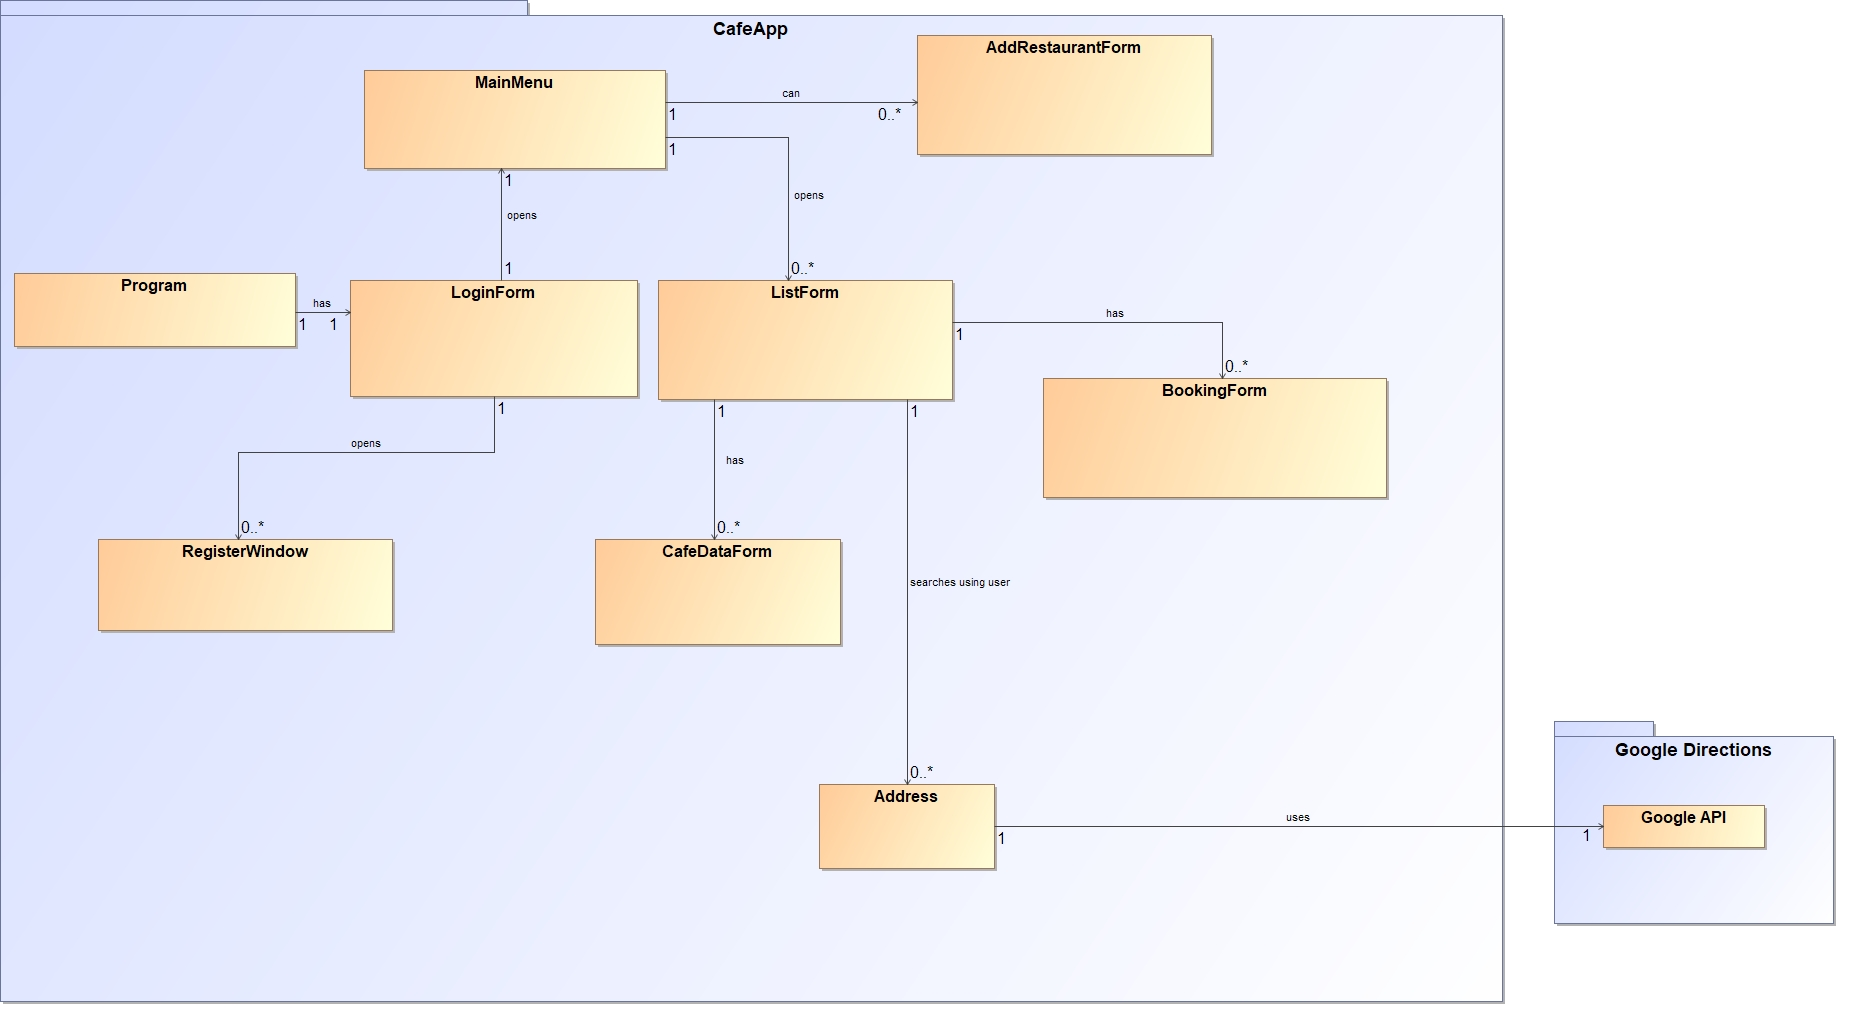
\includegraphics[width=\textwidth,height=\textheight,keepaspectratio]{img/Model} 
    \caption{Klasių diagrama}
    \label{img:Model}
\end{figure}
%1 PAV APRAŠYMAS
Pateiktoje diagramoje yra visos programos sistemos modelis. Programa galima suskirstyti į 3 dalis: vartotojo prisijungimas/registracija prie aplikacijos, kavinių registravimas bei registruotų kavinių sąrašas ir kavinių paieška, rezervavimas ir kavinės informacijos modifikavimas. Apie jas bus plačiau aprašome kitose klasių diagramose.
\pagebreak
%2 PAV APRAŠYMAS

Paleidus programą (2 pav.) vartotojas gali prisijungti arba sukurti naują paskyrą. Mes nusprendėme, kad vartotojui, nuėjus į naujos paskyros langelį nedingtų pradinis langelis. Tokiu būdu vartotojui užsiregistravus bus galima iš karto prisijungti ir atsidurti mūsų programos pagrindiniame langelyje arba sukurti naują paskyrą, jeigu jis būtų nepatenkintas esama paskyra. 
\newline
\newline
\newline
\newline
\newline
\newline
\begin{figure}[H]
    \centering
    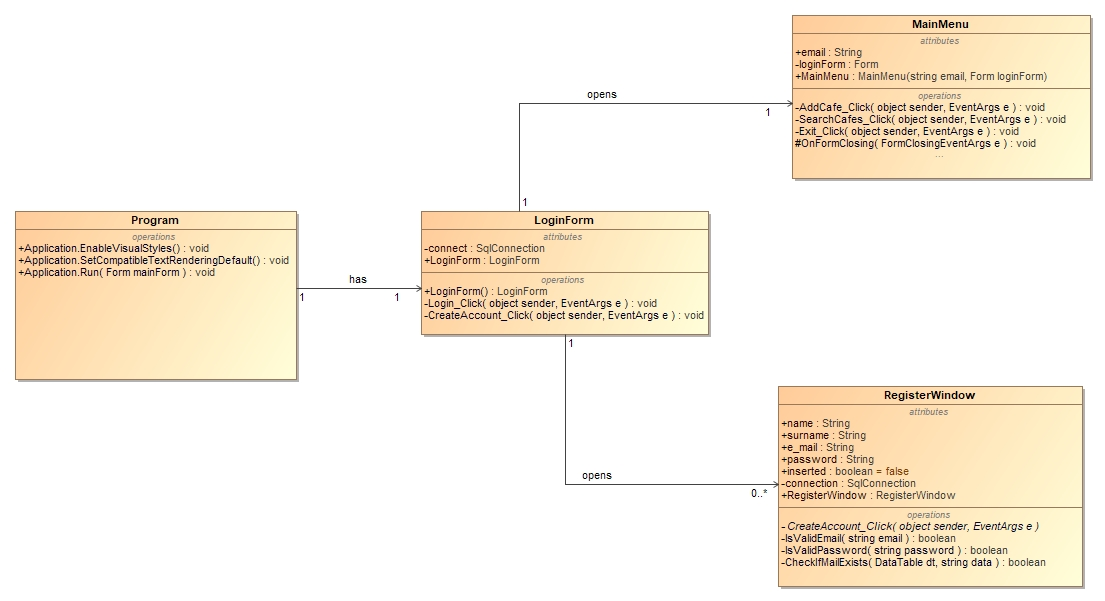
\includegraphics[width=\textwidth,height=\textheight,keepaspectratio]{img/Program_LoginForm_Register_MainMenu} 
    \caption{Programos paleidimo ir vartotojo prisijungimo ir registracijos  klasių diagrama}
    \label{img:Program_LoginForm_Register_MainMenu}
\end{figure}

Kuriant naują paskyrą, privaloma įvesti paštą ir slaptažodį. Bus patikrinama ar įvesti duomenys yra korektiški, taip pat bus patikrinama ar jau nėra tokios sukurtos paskyros su įvestais duomenimis. Prisijungimo metu tikrinama ar yra tokia sukurta paskyra.

\pagebreak
%3 PAV APRAŠMAS
Žemiau pateiktoje klasių diagramoje (3 pav.) pavaizduotos klasės, susijusios su pagrindiniu programos langeliu. Šiame langelyje galima pridėti kavinę į kavinių sąrašą arba atsiverti kavinių sąrašą. Norint pridėti kavinę privaloma nurodyti kavinės pavadinimą, adresą, staliukų skaičių, tvarkaraštį (nuo kada iki kada dirba darbo dienomis, savaitgaliais) ir vartotojo telefono numerį.
\newline
\newline
\newline
\newline
\newline
\newline
\begin{figure}[H]
    \centering
    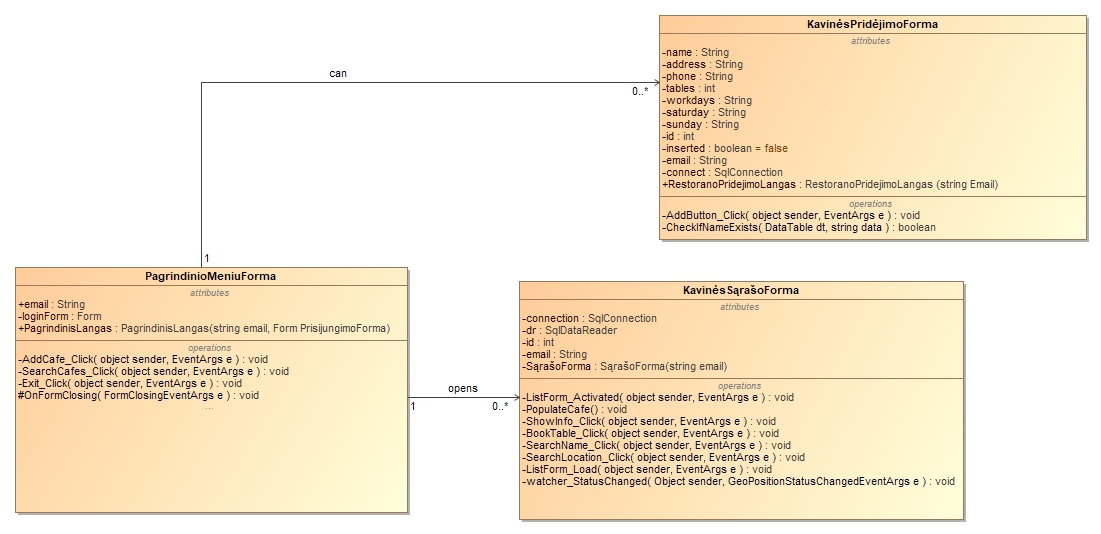
\includegraphics[width=\textwidth,height=\textheight,keepaspectratio]{img/MainMenu_AddRestaurant_ListForm} 
    \caption{kavinių registravimo ir registruotų kavinių sąrašo klasių diagrama}
    \label{img:MainMenu_AddRestaurant_ListForm}
\end{figure}

Kavinės registravimo metu yra patikrinama ar yra kavinė su tokia pačia informacija, kad būtų išvengta dubliavimo.

\pagebreak
%4 PAV APRAŠYMAS
4 pav. klasių diagramoje parodomas kavinių paieška ir kavinės rezervavimas. Mes nusprendėme leisti vartotojui ieškoti norimos kavinės pagal kavinės vardą arba pagal vartotojo esamą vietovę. Taip palengvinama kavinės paieška, jeigu vartotojas žino, jog yra šalia kavinės, bet nežino jos pavadinimo, arba žino kavinės pavadinimą, bet nežino kur ji randasi. Jeigu vartotojas yra ir registruotos kavinės savininkas, jis  gali pakeisti jos vardą, adresą, staliukų skaičių, telefono numerį. Tokiu būdu pataisoma klaidinga registruotos kavinės informacija.
\newline
\newline
\newline
\newline
\newline
\newline
\newline
\newline

\begin{figure}[H]
    \centering
    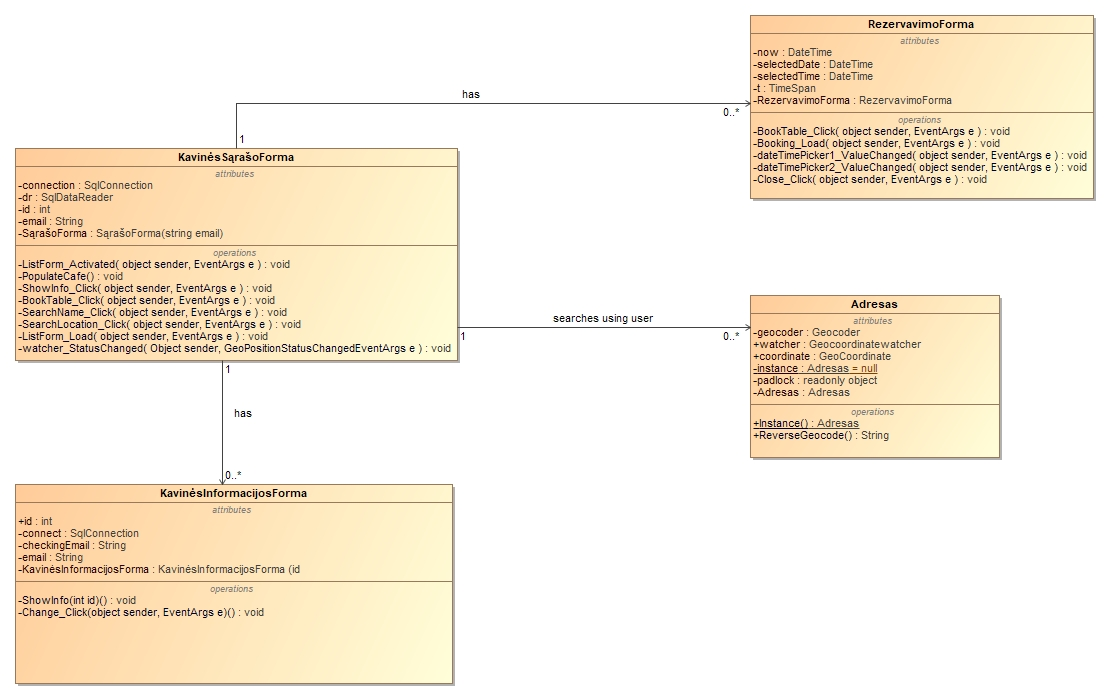
\includegraphics[width=\textwidth,height=\textheight,keepaspectratio]{img/LoginForm_Address_Booking} 
    \caption{kavinių paieškos ir kavininės rezervavimo klasių diagrama}
    \label{img:LoginForm_Address_Booking}
\end{figure}
\pagebreak
%Modes use-cases
\subsection{Užduotys ir jų vykdymo scenarijai (angl. Use-cases)}
Šiame skyriuje bus pavaizduotas mūsų programos užduotys ir jų vykdymo scenarijai.
\subsubsection{Sistemos vykdomos užduotys}

%first figure text
Sistema besinaudojantis vartotojas gali atlikti žemiau pateiktas užduotis. Nusprendėme užduotis išskirstyti į „Paprasto vartotojo“ ir „Restorano savininko“, nes šie agentai turi galimybę atlikti skirtingas užduotis. Restorano savininkas taip pat yra paprastas vartotojas, tačiau savininko statusas leidžia jam tvarkyti tik savo pridėtus restoranus (pvz.: pakeisti restorano informaciją). Paprastas vartotojas taip pat gali tapti restorano savininku, jei prideda savo restoraną. Tai atsispindi žemiau pateiktoje sistemos užduočių diagramoje.

%first picture SystemTasks
\begin{figure}[H]
	\centering
	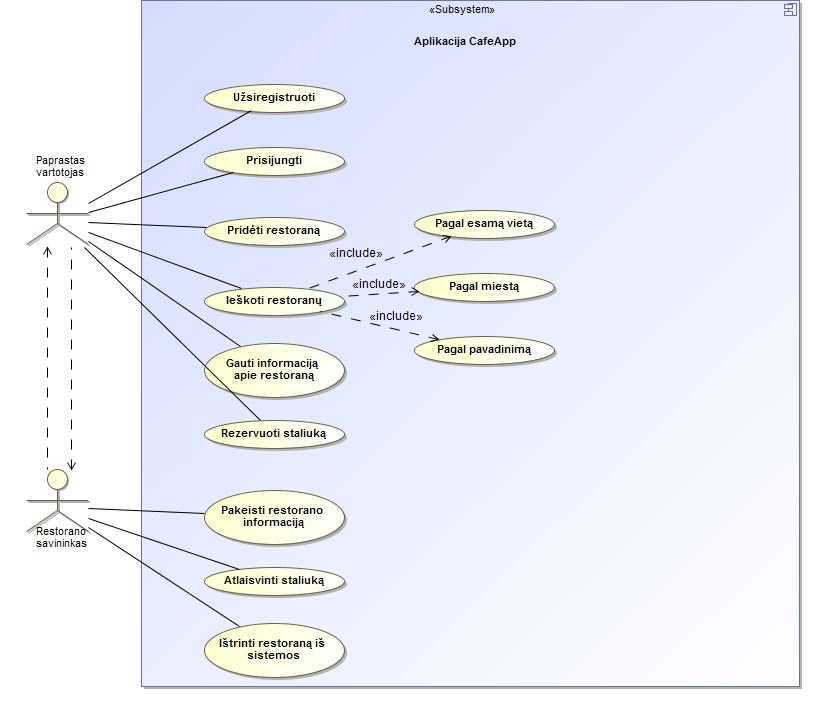
\includegraphics[width=\textwidth,height=\textheight,keepaspectratio]{img/SystemTasks}
	\caption{Sistemos užduočių diagrama}
	\label{img:SystemTasks}
\end{figure}

%second section
\subsubsection{Užduoties „Prisiregistruoti prie sistemos“ vykdymas}
Užduoties „Prisiregistruoti prie sistemos“ sekų diagrama. Vartotojas, naudodamasis GUI, paspaudžia mygtuką „Registruotis“ ir juo iškviečia registracijos formą, kurioje užpildo reikalingus laukus. Duomenys siunčiami kontroleriui, kuris patikrina ar jie tvarkingi (pvz.: ar egzistuoja toks elektroninio pašto adresas), ir iš kontrolerio siunčiama komanda sukurti duomenų bazėje naują įrašą apie vartotoją.

%second figure
\begin{figure}[H]
	\centering
	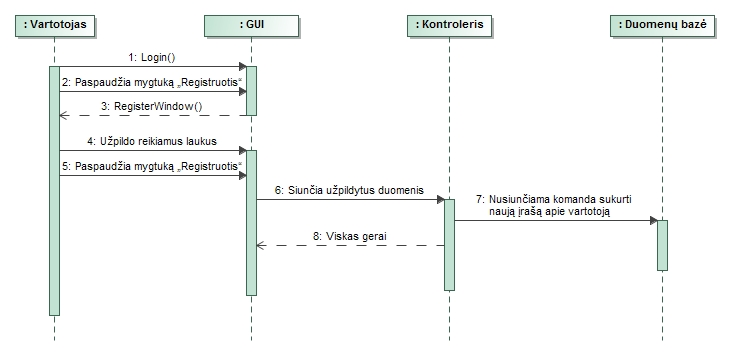
\includegraphics[width=\textwidth,height=\textheight,keepaspectratio]{img/Register}
	\caption{Užduoties „Prisiregistruoti prie sistemos" sekų diagrama}
	\label{img:RegisterTask}
\end{figure}

%third section
\subsubsection{Užduoties „Pridėti naują restoraną“ vykdymas}
Žemiau pateiktoje sekų diagramoje pavaizduotas užduoties „Pridėti naują restoraną“ vykdymas. Vartotojas spaudžia mygtuką „Add a Cafe“ taip iškviesdamas GUI formą, kurią užpildo. Tada paspaudžia mygtuką „Add“ ir duomenys yra validuojami kontroleryje. Jeigu jie neatitinka nustatytų reikalavimų (pvz.: trūksta būtinų užpildyti laukų), vartotojui pranešama ir prašoma pataisyti duomenis. Priešingu atveju, siunčiama užklausa į duomenų bazę, kuri sukuria  naują įrašą, apie pridėtą restoraną, o vartotojas automatiškai tampa restorano savininku.

%third picture
\begin{figure}[H]
	\centering
	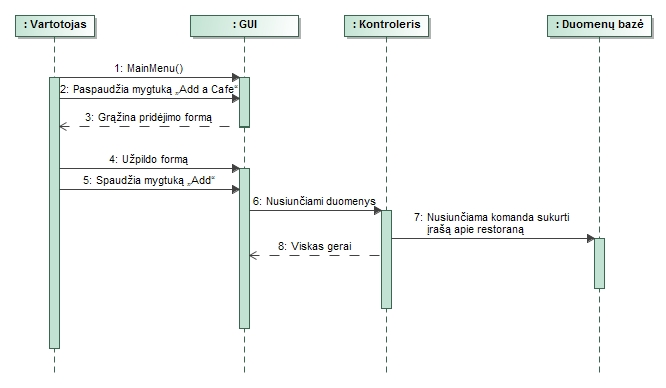
\includegraphics[width=\textwidth,height=\textheight,keepaspectratio]{img/AddRestaurant}
	\caption{Užduoties „Pridėti naują restoraną" sekų diagrama}
	\label{img:AddRestaurant}
\end{figure}

%next section
\subsubsection{Užduoties „Ieškoti restoranų“ vykdymas}
Užduoties „Ieškoti restoranų“ sekų diagrama. Vartotojas paspaudžia mygtuką „Search Cafes“ ir iškviečia naują duomenų formą, kurioje užpildo paieškos kriterijus. Yra numatyti trys kriterijai: pagal esamą vietą, pagal miestą/adresą ir pagal restorano pavadinimą. Duomenys siunčiami kontroleriui, kuris patikrina pateiktus kriterijus, jeigu reikia, nustato esamą vietą, paprašydamas įjungti įrenginio lokaciją. Jeigu viskas yra gerai, siunčiama paieškos užklausa į duomenų bazę ir ji, naudodamasi GUI, pateikia restoranus pagal pasirinktus paieškos laukus. Tai atsispindi žemiau pavaizduotoje sekų diagramoje.

%fourth picture
\begin{figure}[H]
	\centering
	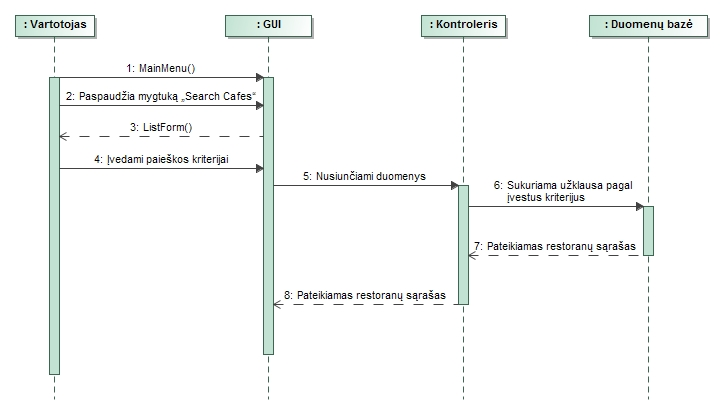
\includegraphics[width=\textwidth,height=\textheight,keepaspectratio]{img/SearchCafes}
	\caption{Užduoties „Ieškoti restoranų" sekų diagrama}
	\label{img:SearchCafes}
\end{figure}

%last section
\subsubsection{Užduoties „Pakeisti restorano informaciją“ vykdymo scenarijus}
Žemiau pavaizduota užduoties „Pakeisti restorano informaciją“ sekų diagrama. Restorano savininkas paspaudžia mygtuką „Search Cafes“ ir juo GUI kreipiasi į duomenų bazę, kuri pateikia visus užregistruotus restoranus. Vykdydamas užduotį „Ieškoti restoranų“ savininkas susiranda savo restoraną, jį pažymėdamas kairiuoju pelės klavišu. Tada paspaudžia mygtuką „Show Info“ ir GUI iškviečia naują formą, kuri kreipiasi į duomenų bazę pagal restorano „ID“ ir parodo informaciją apie restoraną. Joje yra tušti laukai, kuriuos užpildydamas vartotojas gali pakeisti tam tikrą restorano informaciją. Mygtuku „Change“ vartotojas kreipiasi į kontrolerį, kuris siunčia užklausą į duomenų bazę, patikriną, ar būtent šis vartotojas sukūrė įrašą apie restoraną, ir jeigu tai tiesa, vėl kreipiamasi į duomenų bazę - atnaujinti pakeistus duomenis. Jeigu vartotojas neturi teisės keisti informacijai, jam apie tai pranešama.

%last picture
\begin{figure}[H]
	\centering
	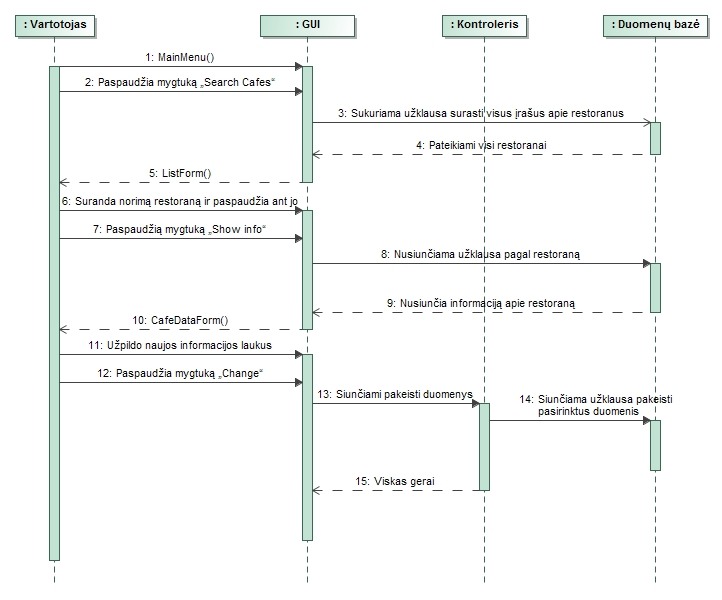
\includegraphics[width=\textwidth,height=\textheight,keepaspectratio]{img/ChangeInfo}
	\caption{Užduoties „Pakeisti restorano informaciją" sekų diagrama}
	\label{img:ChangeInfo}
\end{figure}
%Baigias Modes failai

\subsection{Dinaminis programų sistemos modelis (angl. Process view)}
Šiame skyriuje bus pavaizduotas mūsų programos dinaminis programų sistemos modelis.
\subsubsection{Veiklos diagramos}
\begin{figure}[H]
    \centering
    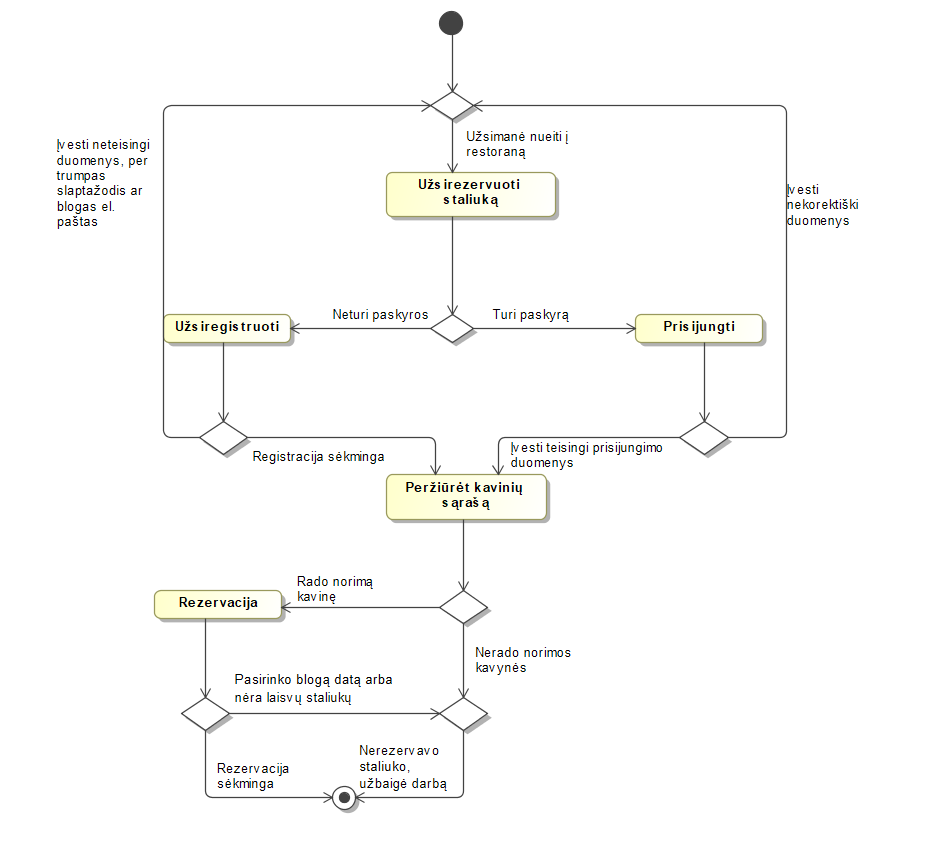
\includegraphics[width=\textwidth,height=\textheight,keepaspectratio]{img/rezerv} 
    \caption{Kavinės rezervacijos veiklos diagrama}
    \label{img:rezerv}
\end{figure}
% Vietoj x įrašyt real sk.
23 pav.   diagramoje nagrinėjami procesai, vykstantys tuo metu, kai vartotojas nori rezervuoti staliuką kavinėje. Rezervacija yra pasiekiama tik po prisijungimo arba užsiregistravimo sistemoje. Vartotojas pamato prisijungimo ir registracijos opcijas tik paleidęs aplikaciją. Būsimas sistemos narys privalo užpildyti registracijos formą, parinkti saugų slaptažodį, bei nurodyti egzistuojantį el. paštą. Užpildžius formą neteisingai, reikia pakeisti netinkamus laukus. Sėkmingai prisijungus prie sistemos, vartotojas gali peržiūrėti aplikacijoje užregistruotų kavinių sąrašą. Jeigu vartotojas randa jam patinkančią kavinę, jis užpildo rezervavimo formą. Jeigu formoje visi laukai yra nurodyti teisingai ir restorane yra laisvų staliukų - rezervacija yra sėkminga. Darbas yra baigiamas tuo metu, kai vartotojas sėkmingai užsirezervavo staliuką, arba nusprendė nutraukt rezervaciją.


\begin{figure}[H]
    \centering
    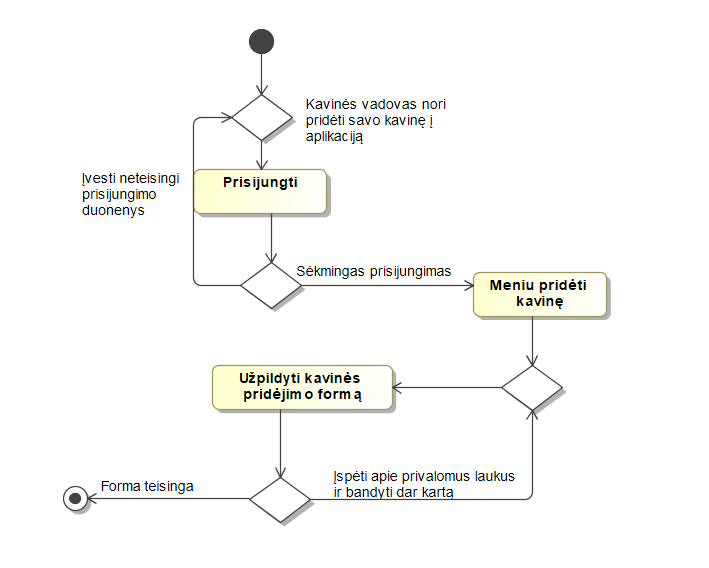
\includegraphics[width=\textwidth,height=\textheight,keepaspectratio]{img/addcafe} 
    \caption{Kavinės pridėjimo prie sistemos veiklos diagrama}
    \label{img:addcafe}
\end{figure}
% Vietoj x įrašyt real sk.
24 pav.   diagramoje nagrinėjami procesai, vykstantys vartotojui į sistemą pridedant kavinę. Norint pridėt kavinę į kavinių sąrašą, vartotojui būtina prisijungti (o neturint prisijungimo - prisiregistruoti) prie sistemos. Prisijungus meniu spaudžiama ant "Add cafe" mygtuko ir užpildoma kavinės pridėjimo formą. Jeigu visi laukai pažymėti "*" (būtini) yra užpildyti - kavinė yra pridedama prie sąrašo. 

\begin{figure}[H]
    \centering
    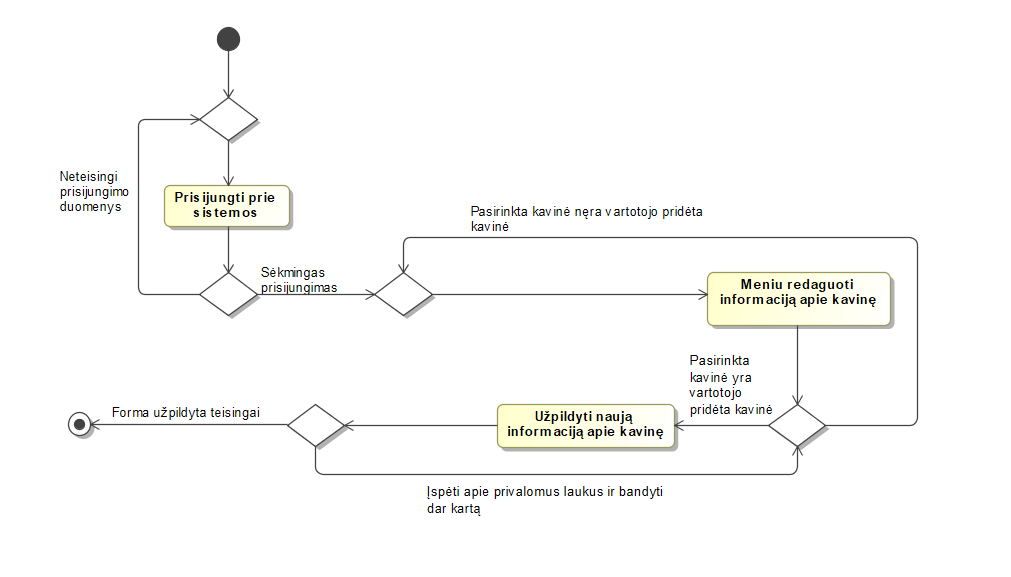
\includegraphics[width=\textwidth,height=\textheight,keepaspectratio]{img/editcafe} 
    \caption{Informacijos apie kavinę redagavimo veiklos diagrama}
    \label{img:editcafe}
\end{figure}
% Vietoj x įrašyt real sk.
25 pav.   diagramoje nagrinėjami procesai, vykstantys vartotojui norint pakeist arba atnaujint informaciją apie kavinę. Norint redaguot kavinės informaciją, vartotojui būtina prisijungti prie sistemos. Vartotojas atidaro visų kavinių sąrašą ir pasirinkus savo kavinė ir paspaudus mygtuką "Show info" jis gauna informacija apie jo kavinę bei apačioje formą, kuria teisingai užpildžius ir paspaudus mygtuką "Change" galima atnaujint/pakeist egzistuojančią informaciją apie kavinę.


\subsection{Programų sistemos išskirstymas tinkle(angl. Deployment view)}
Šiame skyriuje bus pavaizduotas mūsų programos išskirstymas tinkle.
\subsubsection{Komponentų ryšių su artefaktais diagrama}

Žemiau pateiktoje komponentų ryšių su artefaktais diagramoje yra išskirti pagrindiniai sistemos artefaktai. Artefaktus (angl. “artifact”) ir komponentus (angl. “component”) tarpusavyje sieja manifestacijos (angl. “Manifest”) ryšys. Tai reiškia, kad artefakto sudaromoji dalis yra konkretus komponentas.


%Komponentų ryšių su artefaktais diagrama
\begin{figure}[H]
    \centering
    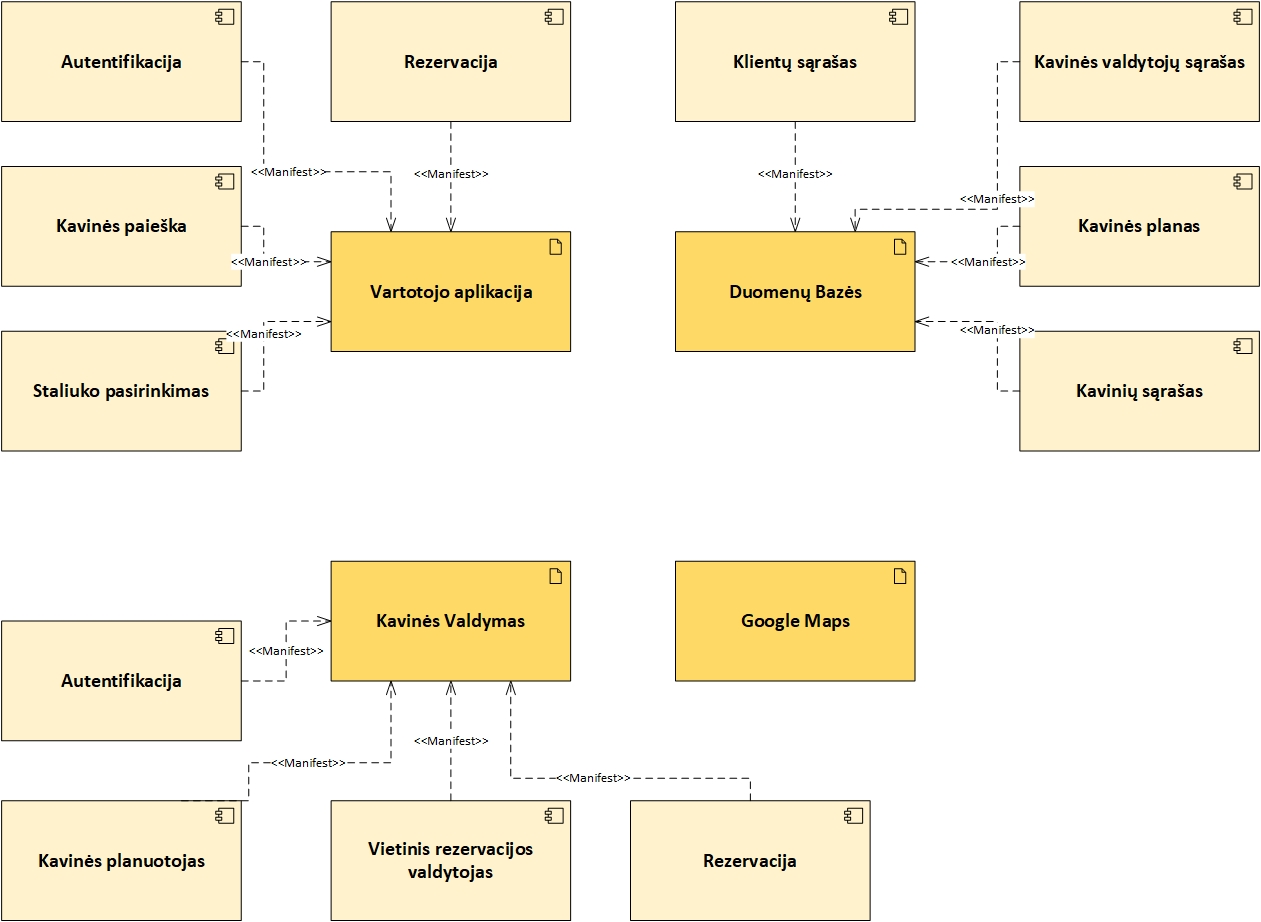
\includegraphics[width=\textwidth,height=\textheight,keepaspectratio]{img/Deployment_diagram1} 
    \caption{Komponentų ryšių su artefaktais diagrama}
    \label{img:Model}
\end{figure}




Visos kavinės programėlės pagrindas susideda iš trijų karkasų: „Registracijos / Prisijungimo sistemos“, „Kavinės pridėjimo sistemos“ ir „Kavinės staliuko rezervacijos sistemos“.

„Registracijos / Prisijungimo sistema“ užtikina kiekvieno vartotojo (kliento ar kavinės savininko) sklandų prisijungimą prie sistemos. Komponentas - „Kontoleris“ užtikina sklandžią registraciją ir prisijungimą prie sistemos. Tai reiškia, kad kiekvieno prisiregistravusiojo duomenys jo deka yra autentiški. Taip pat registracija suteikia galimybę užsiregistruoti kaip klientas arba kavinės savininkas.

„Kavinės pridėjimo Sistema“ - aktuali programėlės vartotojams prisiregistravusiems kaip kavinės savininkas. Ši Sistema užtikina turimų duomenų apie užregistruotas kavinines saugumą. Komponentas - „Kavinės pridėjimas“ leidžia programos vartotojui pridėti kavinę bei detalę jos informaciją. Kavinės informacija dalis yra labai lanksti, ji teikia galimybę pakeisti užregistruotų kavinių pateiktą informaciją: modifikuoti staliukų skaičių, pakeisti kavinės vietą. Sistemos kontroleris patikina, kad nubūtų užregistruojama pasikartojanti inforamcija apie kavines.

Klientams yra prienama „Kavinės staliuko rezervacijos sistema“. Šis karkasas yra nesudėtingas, gali būti laisvai naudojamas, skirtas užtikinti klientų konfortą ir garantuotų rezervacijos stabilumą. Jį sudaro trys pagrindiniai komponentai - kontroleris, Informacija apie kavinę, staliuko rezervacija. Staliuko rezervacija yra esminis komponentas šioje sistemoje. Jis leidžia klientui užsirezervuoti norimą staliuką pasirinktu laiku. Kontroleris užtikina, kad nebūtų suteikiama užsisakyti staliuko tuo pačiu metu kelis kartus skirtingiems klientams. Detalią informaciją apie kavinių sąrašą, jų buvimo vietą, contaktus bei detalesnę informaciją pateikia komponentas pavadinimu - „Informacija apie kavinę“.  


\subsubsection{Mazgų diagrama}

Žemiau pateiktoje mazgų diagramoje yra išskirti fiziniai įrenginiai, reikalingi sistemos darbo palaikymui bei artefaktų pasiskirstymui tarp jų.
%Mazgų diagrama
\begin{figure}[H]
    \centering
    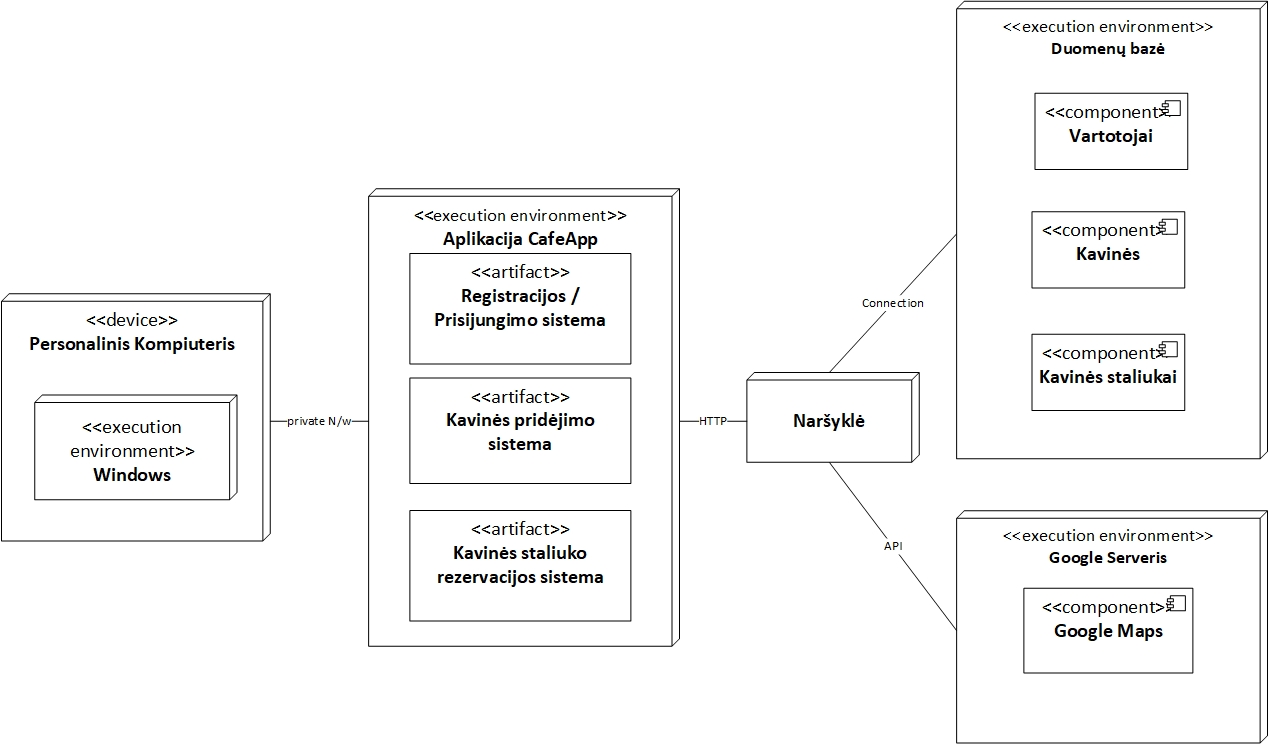
\includegraphics[width=\textwidth,height=\textheight,keepaspectratio]{img/Deployment_diagram2} 
    \caption{Mazgų diagrama}
    \label{img:Model}
\end{figure}


Sistema susideda iš dviejų pagrindinių mazgų Kavinės programėlės ir "Azure" SQL duomenų bazės. Kavinės programėlės visi duomenys yra saugomi serverinėje duomenų bazėje, taip ši programėlė išvengia papidomų duomenų failų, neeikvoja daug kompiuterio atminties ir paspartina procesų darbą. Programa pritaikyta veikti "Windows" platformoje. Vartotojui norint naudotis šia sistema, tereikia atsisiųsti ir įdiegti "Kavinės programėlę" ir turėti prieigą prie Interneto. Taip „Kavinės aplikacija“ pasiekia duomenis iš duomenų bazės, kurioje yra saugoma vartotojų prisijungimai, kavinės duomenys, kavinių staliukų duomenys. Tuo pačiu metu naršyklė kreipiasi į "Google" serverius, siekiant gauti "Google" žemėlapius. Toks sprendimas pasirinktas todėl, kad neužimtų serverio vietos, bei dėl to, kad "Google" riboja prieigą prie savo žemėlapių serviso. 




%KAROLIS KURIMO PJUVIS START
\subsection {Programų sistemos kūrimo pjūvis (angl. Developement view)}
Kūrimo pjūvis išdėstytas “top-down” būdu, t.y. nuo bendresnių
diagramų pereinant iki detalesnių.

\subsubsection{Konteksto diagrama}

\begin {figure}[H]
	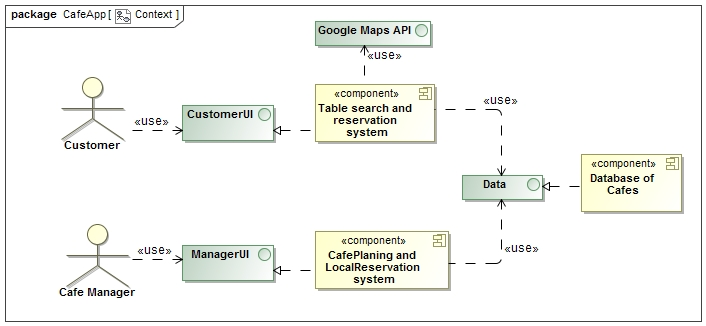
\includegraphics[width=\textwidth,height=\textheight,keepaspectratio]{img/Context}
	\caption{Konteksto komponentų diagrama}
	\label{fig:Context}
\end{figure}

\ref {fig:Context} pav. diagramoje parodomas aukščiausias komponentų struktūros lygis. Klientas (angl. Customer) naudoja Kliento Vartotojo Sąsaja (angl. CustomerUI) kurią gauna iš staliukų paieškos ir rezervacijos sistemos (angl. Table Search and Reservation system) kuri pati naudoja Google Maps API, padedanti atfiltruoti netoliese esančias kavines. \\
Kavinės sąvininkas/vadovas/darbuotojas (diagramoje angl. Cafe Manager) naudoja Vadovo Vartotojo Sąsają (angl. ManagerUI) kurią gauna iš kavinės planavimo ir lokalios rezervacijos sistemos (angl. Cafe Planning and Local Reservation system).\\
Tiek staliukų paieškos ir rezervacijos sistema, tiek kavinės planavimo ir lokalios rezervacijos sistema naudoja duomenis, kuriuos gauna iš Kavinių Duomenų Bazės (angl. Database of Cafes).


\begin{landscape}
\subsubsection{Subsistemų dekompozicija}
	\begin {figure}[H]
		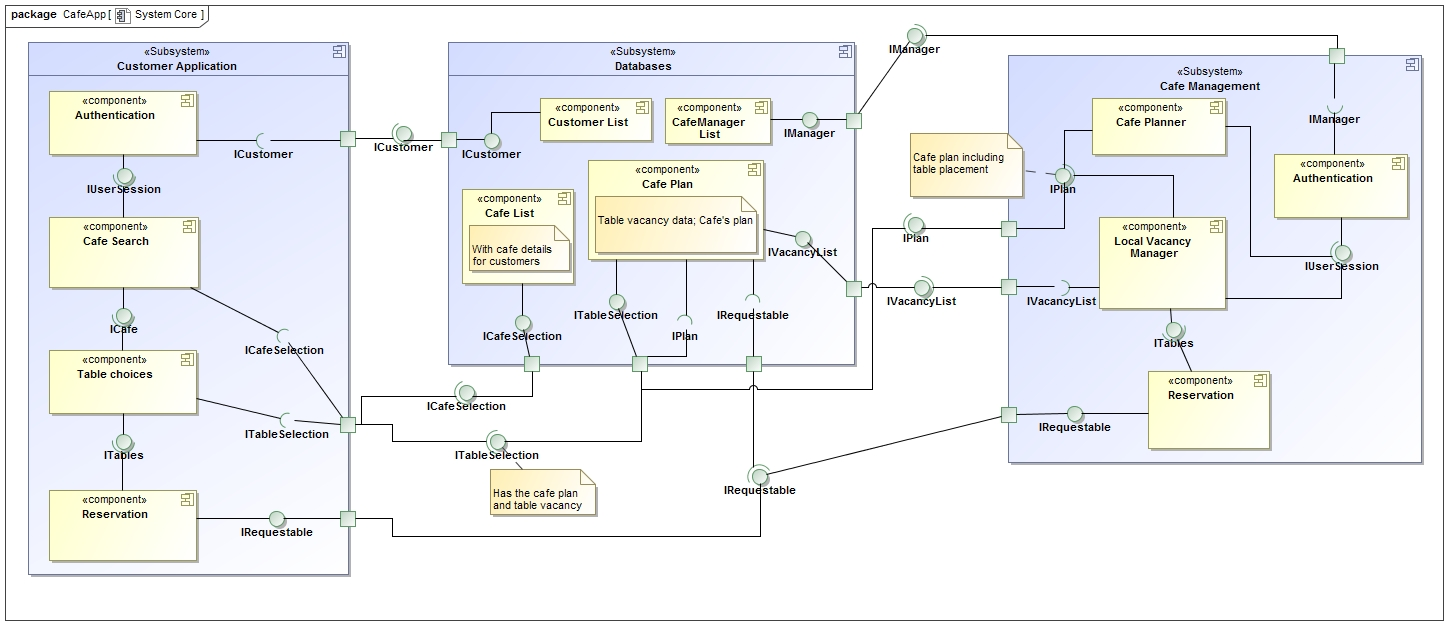
\includegraphics[width=1.67\textwidth,height=1.67\textheight,keepaspectratio]{img/SystemCore}
		\caption{Subsistemų dekompozicijos diagrama}
		\label{fig:System Core}
	\end{figure}
\end{landscape}

\ref {fig:System Core} pav. diagrama atvaizduoja detalų sistemos komponentų struktūros lygį. \ref {fig:System Core} pav. pavaizduotos mėlynai apipavidalintos subsistemos (angl. subsystem) yra \ref {fig:Context} pav. pavaizduoti komponentai:
\begin{itemize}
  \item Vartotojo aplikacija (angl. Customer Application) yra kavinų paieškos ir staliukų rezervacijos sistema;
  \item Kavinės valdymas (angl. Cafe Management) yra kavinės planavimo ir lokalios rezervacijos sistema;
  \item Duomenų bazės (angl. Databases) yra kavinių duomenų bazės.
\end{itemize}
Toliau yra detaliau nagrinėjami šių subsistemų komponentai.\\

\subsubsubsection{Vartotojo aplikacija (angl. Customer Application)}
\begin{itemize}
  \item \textbf{Autentifikacija (angl. Authentication).} Vartotojui sėkmingai prisijungus, iš duomenų bazės klientų sąrašo (angl. Customer List) gaunami įvairūs vartotojo duomenys. Pasinaudojus tais duomenimis pradedama vartotojo sesija (angl. User Session), kurios dėka vartotojas gali naudotis tolesniu programos funkcionalumu.
  \item \textbf{Kavinės(-ių) paieška (angl. Cafe Search).} Kreipiasi į duomenų bazės kavinių sąrašą (angl. Cafe List) ir gauna, pagal vartotojo nurodytą filtrą, kavinių sąrašą su pagrindiniais kavinės duomenimis.
  \item \textbf{Staliuko(-ių) pasirinkimas (angl. Table choices).}  Iš kavinės(-ių) paieškos vartotojui išsirinkus kavinę vykdoma kavinės duomenų (staliuko užimtumo/rezervacijos laiko, kavinės išplanavimo) užklausa į duombazės kavinės plano (angl. Cafe Plan komponentą. Gavus duomenis, vartotojas gali patogiai išsirinkti kurį nors laisvą staliuką konkrečioje kavinės vietoje.
  \item \textbf{Rezervavimas (angl. Reservation).} Iš staliuko pasirinkimo komponento gaunamas norimas rezervuoti staliukas (angl. Table). Vartotojas nurodo rezervavimo laiką-datą. Turint visus rezervacijos duomenis, išsiunčiama rezervavimo užklausa (diagramoje pavaizduota kaip IRequestable) į duomenų bazę, kurioje atsinaujina staliuko būsena iš laisvo į rezervuotą.
\end{itemize}

\subsubsubsection{Kavinės valdymas (angl. Cafe Management)}
\begin{itemize}
  \item \textbf{Autentifikacija (angl. Authentication).} Suvedus teisingus prisijungimo duomenis iš duomenų bazės gaunamas leidimas dirbti su konkrečios kavinės duomenimis.
  \item \textbf{Kavinės topografas (angl. Cafe Planner).} Iš autentikacijos komponento gavus prieinamos kavinės duomenis, leidžia keisti kavinės išplanavimą (tuo pačiu ir staliukų skaičių, išsidėstymą). Išplanavimo duomenys vėliau siunčiami į duomenų bazės kavinės plano (angl. Cafe Plan) komponentą; naudojami vietos užimtumo valdyme.
  \item \textbf{Vietos užimtumo valdymas (angl. Local Vacancy Manager).} Po sėkmingos autentikacijos leidžia stebėti kurie staliukai yra laisvi, kurie užimti, kurie rezervuoti per aplikaciją iš kliento pusės. Taip pat suteikia galimybę rezervuoti arba pažymeti kaip užimtą staliuką iš kavinės pusės.
  \item \textbf{Rezervavimas (angl. Reservation).} Iš Vietos užimtumo valdymo komponentų pasiima duomenis apie staliukų būseną (užimtas, laisvas, rezervuotas, bus-rezervuotas) ir siunčia pasikeitusius duomenis į duomenų bazės kavinės plano (angl. Cafe Plan) komponentą.
\end{itemize}

\subsubsubsection{Duomenų bazė (angl. Databases)}
\begin{itemize}
  \item \textbf{Klientų sąrašas (angl. Customer List).} Suteikia galimybę autentifikuoti vartotoją, laiko papildomus duomenis apie jį.
  \item \textbf{Kavinės valdytojų (angl. Cafe Manager List).} Suteikia galimybę autentifikuoti sąvininką/vadovą/darbuotoją, taip pat pateikia duomenis kokiai kavinei dirba šis asmuo (vėliau ši informacija reikalinga žinoti kurios kavinės duomenys modifikuojami).
  \item \textbf{Kavinių sąrašas (angl. Cafe List).} Klientui ieškant kavinės, pateikia atfiltruotą kavinių sąrašą, kartu su kavinės reprezentacine informacija (užimtumas, darbo valandos, reitingas ir pan.).
  \item \textbf{Kavinės(-ių) planas (angl. Cafe Plan).} Laiko visa svarbiausią informaciją apie kavines:
  	\begin{itemize}
  	\item Išplanavimas, staliukų išsidėstymas ir kiti tos srities duomenys ir jų pakeitimai gaunami iš kavinės valdymo (angl. Cafe Management) subsistemos kavinės topografo (angl. Cafe Planner) komponento.
  	\item Staliukų būsena - laisva/rezervuota - pakeičiama gavus prašymą (angl. Request) iš kliento aplikacijos (angl. Customer Application) subsistemos. Įvairesnius pakeitimus gali atlikti prašymai iš kavinės valdymo (angl. Cafe Management) subsistemos: atlaisvinti, užimti, rezervuoti, atšaukti rezervaciją.
  	\item Kavinės išplanavimas, staliukų būsena ir išdėstymo duomenys perduodami gavus prašymą (angl. Request) iš kliento aplikacijos (angl. Customer Application) subsistemos staliuko(-ių) pasirinkimo (angl. Table choices) komponento.
  	\item Konkrečios kavinės staliukų užimtumui pasikeitus nauji duomenys yra siunčiami į tos kavinės kavinės valdymo (angl. Cafe Management) subsistemos vietos užimtumo valdymo (angl. Local Vacancy Manager) komponentą, kurio dėka sąvininkas/vadovas/darbuotojas mato, jog klientas užsirezervavo staliuką.
  	\end{itemize}
\end{itemize}

%KAROLIS KURIMO PJUVIS END

\sectionnonum{Išvados}
Dokumento parengimas palengvina sistemos prototipo kūrimą bei tobulinimą. Jis užtikrina
sistemos lankstumą, plečiamumą ir darbo vykdymo efektyvumą. Parengus eskizinį projektą galima
įsitikinti, kad sistema yra įgyvendinama ir esminių kliūčių jos sukūrimui nėra.

%?SITO REIKIA?

\begin{landscape}
\section{Priedai}
	\begin {figure}[H]
		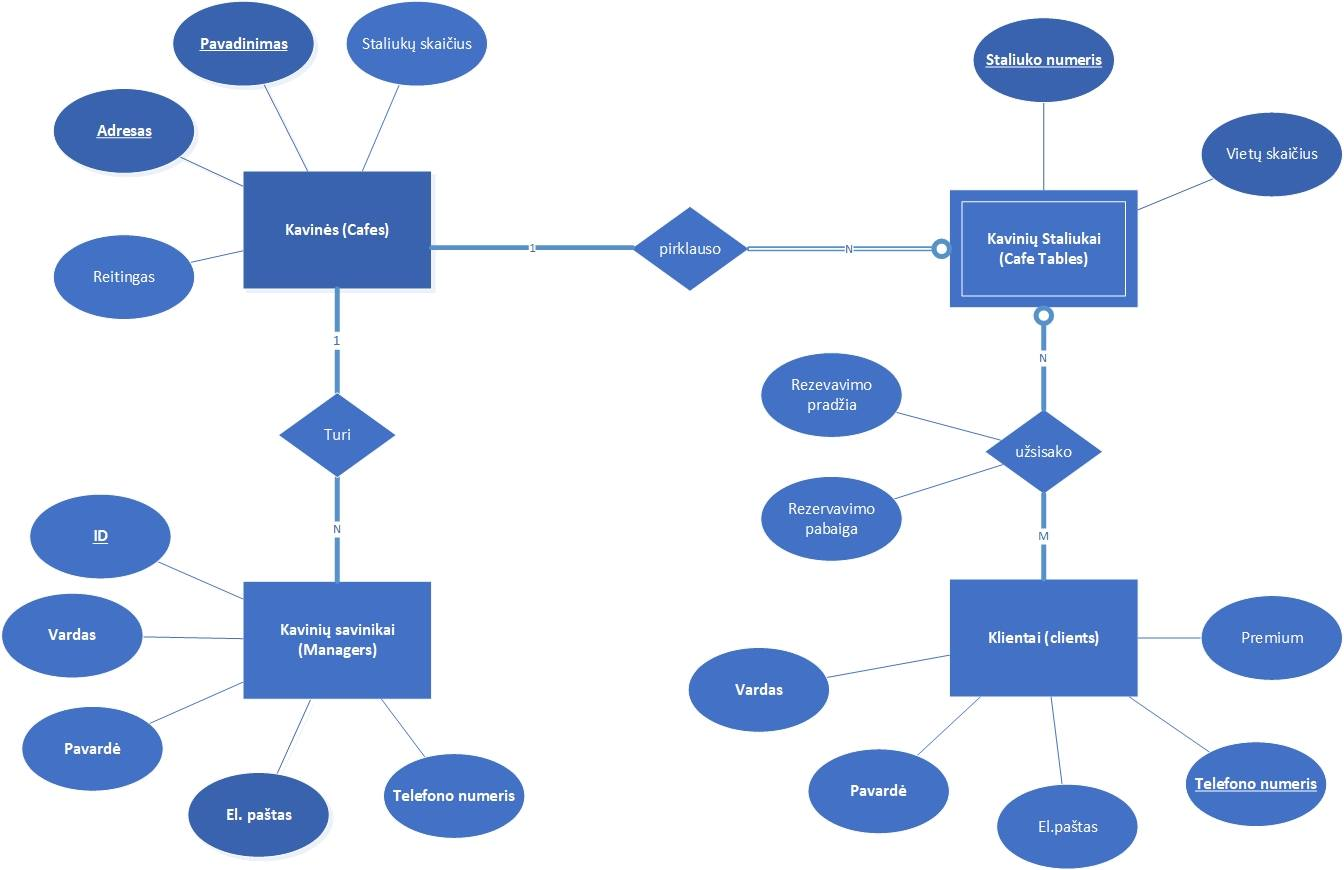
\includegraphics[width=1.3\textwidth,height=1.4\textheight,keepaspectratio]{img/ER}
		\caption{Duomenų bazės E-R diagrama}
		\label{fig:ER}
	\end{figure}
	
	\begin {figure}
		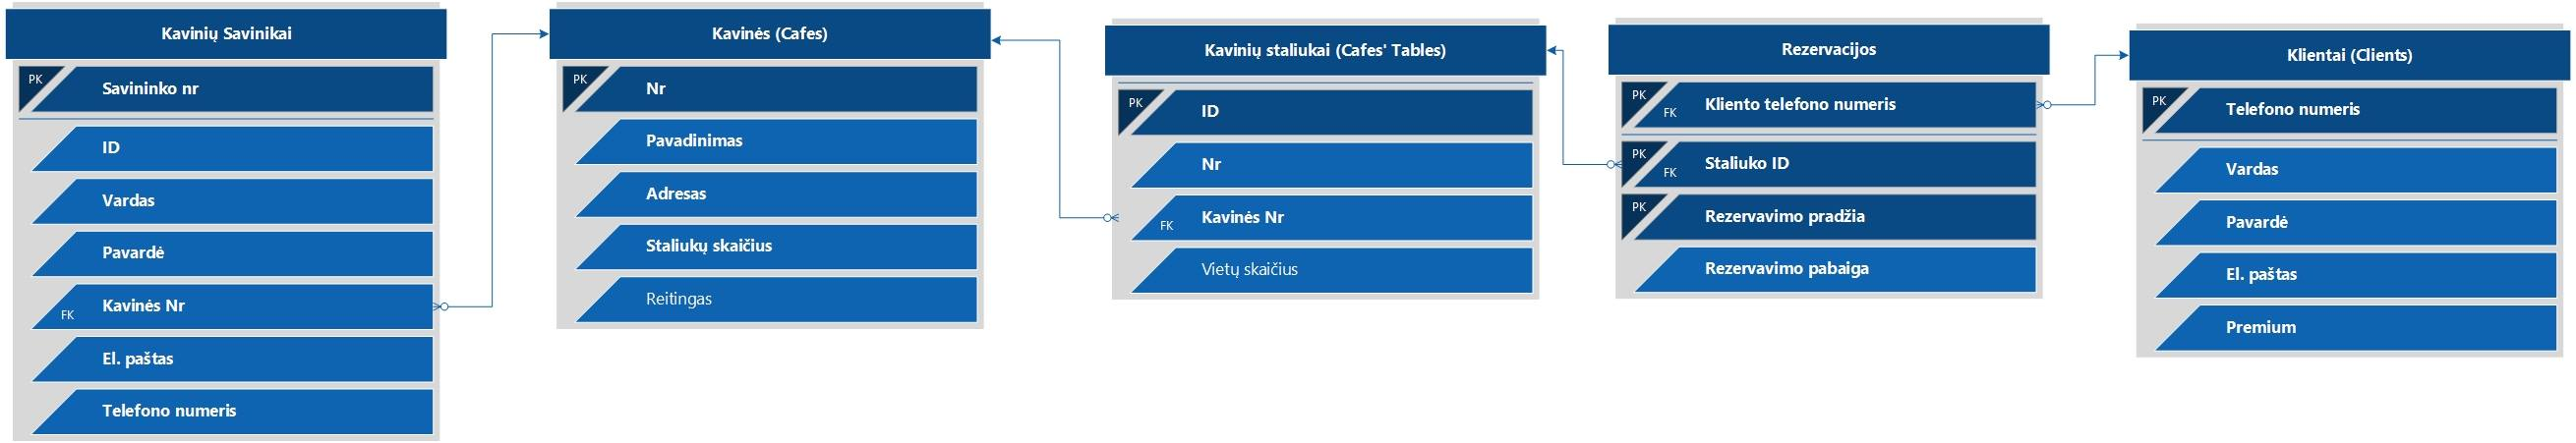
\includegraphics[width=1.5\textwidth,height=1.65\textheight,keepaspectratio]{img/lenteles}
		\caption{Duomenų bazės lentelės}
		\label{fig:lenteles}
	\end{figure}
\end{landscape}

\end{document}
